\documentclass{fhnwreport}
\usepackage[ngerman]{babel}
\usepackage[T1]{fontenc}
\usepackage[utf8]{inputenc}
\usepackage[T1]{fontenc}
\usepackage{subfigure}
\usepackage{tikz}
\usepackage{amsmath}
\numberwithin{equation}{section}
\usetikzlibrary{arrows}
\usepackage{lmodern}   %Type1-Schriftart für nicht-englische Texte
\usepackage{float}
\usepackage{color}

\title{
  \textsc{Fachbericht}\\[2ex]
  \textsc{FS18 - Pro4E - Team 5}  }
\bibliographystyle{fhnwreport/IEEEtran}  

\begin{document}
\maketitle

\textsc{%
\begin{tabbing}
Auftraggeber: \hspace{4em} \= H. Gysin \\[2ex]
\> J. Kalbermatter \\ [2ex]\\
Betreuer:  \>  M. Meier\\[2ex]
\> A. Gertiser \\[2ex]
\> R. Dubach \\[2ex]
\> B. Domenghino\\[2ex]
\> P. Schleuniger \\[2ex]\\
Projektleitung: \> Simon Zoller\\[2ex]\\
Teammitglieder: \> Severin Hunziker\\[2ex]
\> Mischa Knupfer\\[2ex]
\> Lukas Loosli\\[2ex]
\> Josha Giambonini\\[2ex]
\> Elias von Däniken\\[2ex]
\> Gianluca Picciola\\[2ex]\\
Studiengang: \> Elektro- und Informationstechnik\\[2ex]
\end{tabbing}
}


\hbox{}
\clearpage


%%%%%%%%%%%%%%%%%%%Abstract%%%%%%%%%%%%%%%%%%%%%%%

\section*{Abstract}\label{sec:abstract}
Aimlessly wandering around a museum because of too little knowledge is one of the main negative reactions to a museum visit. That’s why no one can remember an individual work of art. To counteract this, an audio guide called Dōjō was designed to provide visitors with key information about a work of art so they can enjoy their visit more. This project should design the circuits for this Dōjō, which electronically recognises the artwork the visitor is standing in front of. Audio information stored on an internal SD-Card over a Class-D Amplifier is provided through an integrated bone sound sensor produced by adafruit. Buttons for audio control have also been integrated. In addition, the Dōjō allows the visitor to \glqq like\grqq an artwork by simply pressing a button. Information about these \glqq liked\grqq works are made available to the visitors either by email or a hardcopy is provided at the end of their visit. Each work of art has a Bluetooth Low Energy (BLE) Beacon that continuously sends its ID to the Dōjō. The Dōjō’s internal microcontroller (nrf52832) then scans for this BLE-Signals and plays the file that belongs to the ID with the strongest signal. The Dōjō can identify beacons at XX meters. The inductive rechargeable battery has a capacity of 800mAh and can provide energy for about 6 hours when the Dojo is playing audiofiles and be recharged in normal charging mode within 13 hours. To protect the battery from damage, a deep discharge protection turns off the Dōjō when the battery is under 3V of its nominal voltage.\\[0.25cm]
Key Words: audio guide, Bluetooth low energy, inductive charge, bone sound sensor
\newpage

%%%%%%%%%%%%%%%%%%%%%%%%%%%%%%%%%%%%%%%%%%%%%%%%%%%
\setcounter{tocdepth}{2} 
\tableofcontents
\newpage

%Input Files
%%%%%%%%%%%%%%%%%%%%%%%%%%%%%%%%%%%%%%%%%%%%%%%%%%%%%%%%
\section{Einleitung}\label{sec:einleitung}
Zielloses Umherwandern und zu wenig Wissen über das Besondere an der Kunst sind nur einige Gründe weshalb bei einem Museumsbesuch oft der Besuch selbst mehr in Erinnerung bleibt als die eigentlichen Kunstobjekte. Um diesem Problem entgegenzuwirken, hat Frau J. Kalbermatter das Gehäuse eines modernen Audioguides entwickelt und sich dazu ein funktionales Konzept ausgedacht. Dieser Audioguide, Dōjō genannt, soll Kunstobjekte drahtlos erkennen und darüber gespeicherte Informationen via Körperschalltechnik zum Museumsbesucher bringen. Dazu muss sich der Benutzer das Ende des stabförmigen Audioguides hinter das Ohr halten. Dank der Informationsübertragung via Körperschall und dem Verzicht auf Kopfhörer, erfüllt der Dōjō höchste Hygieneansprüche, was die Benutzung angenehmer macht. Weiter soll der Audioguide auch als Ticket fungieren und die Zutrittsberechtigung regeln. Das Drücken einer implementierten \glqq Like\grqq-Taste soll vermerken, welche Kunstobjekte dem Besucher gefallen haben. Das ermöglicht es, die Informationen über ein interessantes Kunstobjekt am Ende des Besuchs in Form einer Broschüre oder per E-Mail an den Besucher zu übergeben. Mit diesen Funktionen wird der Dōjō den Museumsbesuch hygienisch und angenehmer gestalten. Ausserdem wird er helfen, das Allgemeinwissen zu verbessern. Dadurch werden die Kunstobjekte und nicht der Besuch selbst zu einem unvergesslichen Erlebnis werden.\\
Ziel im Projekt 4 im Studiengang Elektro- und Informationstechnik an der Fachhochschule Nordwestschweiz war es deshalb, das funktionelle Konzept von Frau Kalbermatter durch die Verwendung von elektrotechnischen Bauteilen zu realisieren. Dazu wurde die drahtlose Erkennung der Kunstobjekte mittels Bluetooth Low Energy (BLE) Beacons erreicht. Genannte Beacons müssen in unmittelbare Nähe der Kunstobjekte angebracht sein. Die Informationen zu den Kunstobjekten wurden als Audiofiles auf einer herausnehmbaren SD-Karte gespeichert und werden zum Abspielen via PWM-Ausgang des Mikrokontrollers (nRF52832) über einen Klasse D Verstärker auf den Knochenschallaktor gegeben. Tasten für die Wiedergabekontrolle (Start, Stopp, Lauter, Leiser) wurden implementiert sowie die erwähnte \glqq Like\grqq -Taste. Ausserdem verfügt der Dōjō über einen Li-Ionen-Akku, welcher induktiv geladen wird. Damit der Dōjō gänzlich drahtlos bleibt, erfolgen Datendownload und Konfiguration ebenso über Bluetooth. Der integrierte Mikrokontroller beinhaltet die Software und übernimmt somit die Erkennung, Ansteuerung und Koordination der Hardware.\\
Es wurde ein Prototyp der Elektronik realisiert. Er kann zu XXX verschiedenen Sprachen XXX Stunden Audioausgabe speichern. Die Ansteuerung der Audiofiles erfolgt über Bluetooth-Beacons, welche bis zu einer Distanz von XXX m erkennt werden. Die eingebaute «Like»-Taste ermöglicht, favorisierte Kunstobjekte zu vermerken und die dazugehörigen Informationen am Ende des Besuches digital oder in Form einer Broschüre beim Ausgang als Erinnerung mitzunehmen. Ausserdem besitzt der Dōjō einen integrierten Akku mit einer Kapazität von XXX mAh, welcher bei pausenloser Audioausgabe genug Energie für XXX Stunden liefert. Die Induktionsladung lädt den Akku zu 100\% innert XXX Stunden. Ausserdem sorgt ein Tiefenentladungsschutz dafür, dass der Dōjō bei XXX\% Akkuladestand ausgeschaltet wird um den Akku vor Schäden zu bewahren.\\
Der nachfolgende Bericht umfasst drei Hauptbereiche. Der erste Bereich (Kapitel 2) umfasst das Gesamtkonzept, welcher die gesamte Anwendung auslegt. Die nachfolgenden zwei Hauptbereiche sind in Hardware (Kapitel 3) und Software (Kapitel 4) gegliedert. Die Hardware teil sich wiederum in die Themengebiete Energieübertragung (Kapitel 3.1), Energiespeicherung (Kapitel 3.2) und Audioausgabe über den Knochenschallaktor (Kapitel 3.5) auf. Die Software beinhaltet die Unterbereiche der State Machine (Kapitel 4.1), Bluetooth (Kapitel 4.3), sowie die gesamte Programmstruktur der SD-Karte (Kapitel 4.4) und Audioausgabe über PWM (Kapitel 4.5). In Kapitel 5 befindet sich die Validierung.\\

\newpage
\section{Gesamtkonzept}\label{sec:gesamtkonzept}
Bevor auf die einzelnen Komponenten des Dōjōs eingegangen werden kann, ist ein Einblick in das Gesamtkonzept notwendig. Hauptbestandteil werden in diesem Kapitel der Aufbau, die Funktionsweise des Gerätes wie auch die Anwendung im Museum sein. Beim Aufbau ist die Kommunikation der einzelnen Komponenten untereinander ersichtlich. Dieser Abschnitt wird durch die jeweiligen Funktionsweisen abgerundet. Der letzte Teil gibt einen Einblick in die Anwendung vor und während dem Museumsbesuch und welche technischen Möglichkeiten dem Besucher zur Verfügung stehen.
\subsection{Funktionsweise}


\subsection{Anwendung}\label{sec:ladeablauf}
Nachdem die ursprüngliche Idee und die Unterteilung zwischen Betreiber und User gemacht wurde, kann nun die Betriebsebene erläutert werden.
Um einen lückenlosen Betrieb zu gewährleisten, ist ein Ablauf für den Gebrauch des Dōjō notwendig. Dieser Ablauf kann zusammenfassend in vier Schritte unterteilt werden und ist nachfolgend in Abbildung \ref{fig:Anwendungsablauf Dojo} ersichtlich.

\begin{figure}[H]
	\begin{center}
		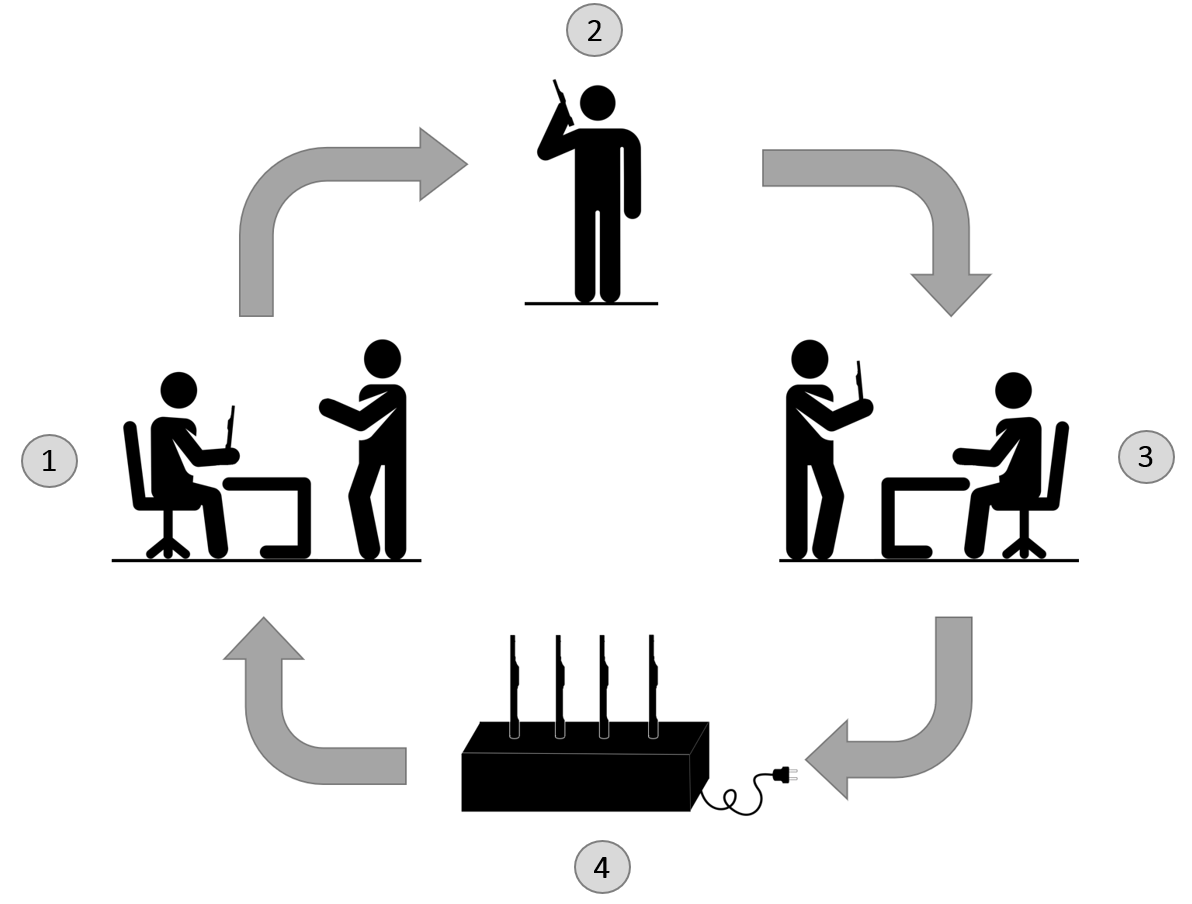
\includegraphics[width=140mm]{data/Ladezyklus.png}
		\caption[Anwendungsablauf des Dojos]{Anwendungsablauf} %picture caption
		\label{fig:Anwendungsablauf Dojo}
	\end{center}
\end{figure}

Der erste Schritt beinhaltet die Ausgabe des Dōjōs am Empfang. Hierbei wird festgelegt zu welchen Bereichen der Besucher Zutritt erhalten soll. Dies ist abhängig von den Wünschen des Besuchers. Die Auswahl der Sprache wird nachfolgend im Abschnitt \nameref{sec:sprachauswahl} beschrieben. Zu beachten gilt es, dass jeweils die Geräte ausgegeben werden, welche sich am längsten in der Ladestation (Schritt 4) befinden. Hierbei hilft eine Signal-LED am Dojo, welche den Ladestatus gemäss definiertem Farbschema wiederspiegelt. Ein lückenloser Betrieb wird erreicht, wenn die Stückzahl der Audio-Guide Geräte in etwa der Anzahl der Besucher pro Tag entspricht.
\\
\\
In Schritt 2 befindet sich der Besucher auf dem Rundgang mit dem Dōjō als Audio-Guide. Der Nutzer hat hierbei die Möglichkeit während dem Rundgang Bilder zu \glqq liken\grqq . Weitere Funktionen und die Bedienung des Dojos selber, ist im vorherigen Unterkapitel \ref{sec:funktionsweise} beschrieben.
\\
\\
Die Abgabe erfolgt in Schritt 3. Hier hat der Besucher die Möglichkeit \glqq gelikte\grqq Bilder als Broschüre zu erhalten oder diese per Mail zu erhalten. Das entgegengenommene Dōjō kann für den nächsten Besucher gereinigt werden.
\\
\\
Sobald das Dōjō entgegengenommen wurde und alle benötigten Informationen (\glqq likes\grqq) extrahiert wurden, wird es wie in Schritt 4 ersichtlich aufgeladen. Hierfür ist eine induktive Ladestation notwendig, wobei die Dōjōs lediglich in die dafür vorgesehenen Ladebuchsen gesteckt werden. Zur Signalisation des Ladevorganges dient eine in jedem Gerät eingebaute Signal-LED, welche bei Spannungsversorgung zu leuchten beginnt.
\\
\\
\subsubsection*{Sprachauswahl} \label{sec:sprachauswahl}

Die Sprachauswahl wird durch den Besucher selbst eingestellt. Hierbei stehen ihm vier Bluetooth-Beacons zur Verfügung, zu welchen er sein Dōjō hinhalten kann. Die gewünschte Sprache ist hierbei durch die Landesflagge gekennzeichnet. Ein Beispiel einer solchen Anwendung ist nachfolgend in Abbildung \ref{fig:SprachauswahlBeacon} ersichtlich.

\begin{figure}[H]
	\begin{center}
		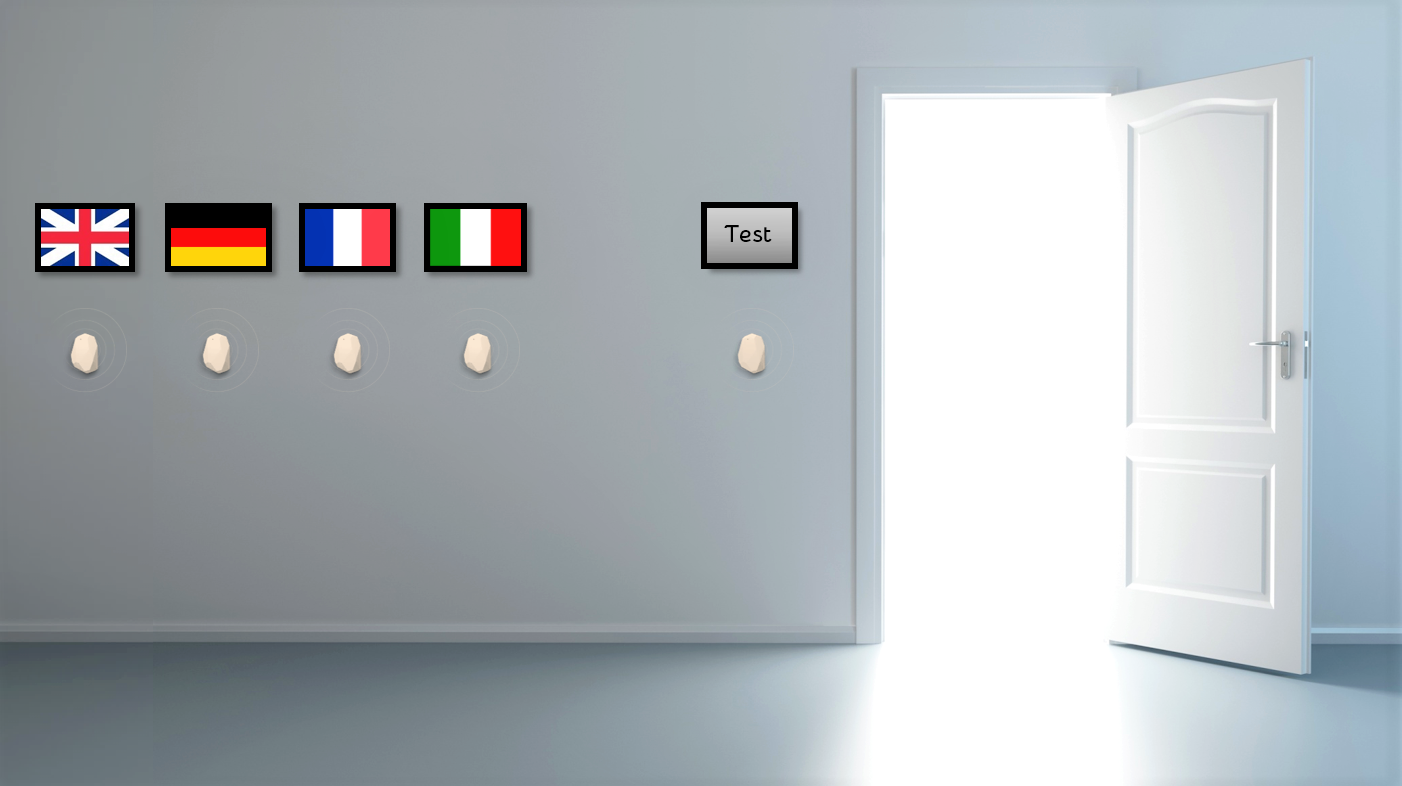
\includegraphics[width=140mm]{data/BeaconSpracherkennung.png}
		\caption[Sprachauswahl mittels Bluetooth-Beacon]{Sprachauswahl mittels Bluetooth-Beacon} %picture caption
		\label{fig:SprachauswahlBeacon}
	\end{center}
\end{figure}

Es ist ersichtlich, dass eine Auswahl aus vier Sprachen möglich ist. Um die gewünschte Sprache auf dem Gerät zu aktivieren, muss der Dōjō an den jeweiligen Sprachbeacon gehalten werden und gleichzeitig die Playtaste gedrückt werden. Wurde die Sprache erfolgreich ausgewählt, wird ein kurzes Audio-Sample mit der gewählten Sprache abgespielt. Diese kurze Sprachausgabe ist lediglich für die Gewissheit des Besuchers ob die richtige Sprache ausgewählt wurde. Sobald die gewünschte Sprache geladen und getestet wurde, kann der Museumsbesuch gestartet werden.

\newpage
\section{Hardware}\label{sec:hardware}


\subsection{Induktive Ladung}\label{sec:energieuebertragung}

Der Dōjō wird mit Hilfe des Induktionsprinzips geladen. Der Ladeprozess wird gestartet, sobald der Dōjō auf die Ladestation gestellt wird. Beim Induktionsprinzip wird die Energie mithilfe von Spulen über eine kurze Distanz zwischen zwei Schaltungen transportiert. Die erste Schaltung, von welcher aus die Energie gesendet wird, wird Transceiver genannt. Diese Schaltung besteht aus einem Pulsgenerator, mit welchem das LC-Glied gepulst wird. Sie macht den Hauptanteil einer solchen Induktiven Ladeschaltung aus. Die zweite Schaltung, welche die Energie des Transceivers empfängt, wird Receiver genannt und besteht ebenfalls aus einem LC-Glied mit einem Gleichtrichter. Nachfolgend werden beide Teile der Schaltung beschrieben.

\subsubsection*{Tranceiver}
Der Pulsgenerator wird einer Timer-Schaltung umgesetzt. Verwendet wird hierbei das elektronische Bauelement NE555. Dieses bietet den Vorteil, dass das notwendige Pulssignal für die Übertragung einfach erstellt und verändert werden kann. Der NE555 enthält eine monolithisch integrierte Zeitgeberschaltung, die sich aufgrund ihrer Eigenschaften als Taktgeber, Oszillator und für Zeitverzögerungen verwenden lässt. Bevor der Timer zu schalten beginnt, müssen verschiedene Spannungsschwellen erreicht werden. Diese lassen sich durch extern angeschlossene Widerstände und Kondensatoren einstellen. Massgebend für die Veränderung der Pulsdauer, Frequenz und des Duty-Cycles sind die Verhältnisse der Komponenten. Das entstandene Pulssignal wird schlussendlich an das LC-Glied gegeben. Dafür wird das LC-Glied an die Versorgungsspannung gehängt und in Serie dazu der Collectoranschluss eines 2N3055 Leistungs NPN-Transistor angeschlossen. An dessen Emitter wird nun ein Niederohmiger Widerstand auf $GND$ gehängt, wobei die über ihm abfallenden Spannung von einem weiteren Transistor überwacht wird und somit den Strom begrenzt. Dieser \glqq 2N2222 Strombegrenzungs-Transistor\grqq wird zwischen dem Pulssignal, welches den Leistungs-Transistor steuert, und GND gehängt. Wird nun der Strom und somit auch die Spannung über dem Widerstand zu hoch, so schliesst der \glqq 2N2222 Strombegrenzungs-Transistor\grqq das Pulssignal kurz, wodurch der 2N3055 Leistungstransistor nicht mehr sauber durchgesteuert wird und dadurch den Strom begrenzt. Die Strombegrenzung ist abhängig von der verwendeten Peripherie des LC-Gliedes. Es gilt zu beachten, dass die Spule durch ihre kleine Bauform weniger Strom verträgt als der Leistungstransistor. In unserem Fall liegt der maximal zulässige Strom für die Spule bei $0.6A$. Bei der Wahl von grösseren Spulen muss jedoch darauf geachtet werden, dass die Begrenzung von 15A nicht überschritten wird, da dies die Belastungsgrenze für den 2N3055 Leistungstransistor ist.
 
Das Pulssignal selber muss verschiedene Kriterien erfüllen. Zum einen sollte der Duty Cycle so nahe wie möglich an $50\%$ sein. Um dies zu erreichen muss $R2 >> R1$ gelten. Das andere Kriterium ist die Erreichung der Resonanzfrequenz des LC-Gliedes. Um das Pulssignal optimal einzustellen, können folgende Richtlinien betrachtet werden:
\begin{description}
	\item [$\cdot$ C] beeinflusst die Zeiten (Frequenz/High-Time/Low-Time)
	\item [$\cdot$ R$_{1}$] beeinflusst die High-Time, lässt jedoch die Low-Time unverändert.
	\item [$\cdot$ R$_{2}$ ] beeinflusst die High- und Low-Time und beeinflusst somit den Duty Cycle.
\end{description}

Die verwendeten Komponenten $C$, $R_{1}$ und $R_{2}$ wurden durch nachfolgende Formeln \ref{eq:TimerF} bis \ref{eq:TimerR2} berechnet. 

<<<<<<< HEAD
\begin{equation}\label{eq: Timer555 F}
F=1/T= 1.44/((R1+R2*2)*C)
\end{equation}
\begin{equation}\label{eq: Timer555 TL}
TL= 0.693*R*C
\end{equation}
\begin{equation}\label{eq: Timer555 TH}
TH= 0.693*(R1+R2)*C
\end{equation}
\begin{equation}\label{eq: Timer555 D}
D= Duty Cycle= (R1+R2)/(R1+2*R2)
\end{equation}
\begin{equation}\label{eq: Timer555 R1}
R1= 1.44**(2*D-1)/(F*C)
\end{equation}
\begin{equation}\label{eq: Timer555 R2}
R2= 1.44*(1-D)/(F*C)
=======
\begin{equation}\label{eq:TimerF}
F=\dfrac{1}{T}=\frac{1.44}{(R_{1}+(R_{2}\cdot 2))\cdot C}
>>>>>>> bf25fa5cc30d7cbbed361af39edc0146dab9a6b3
\end{equation} 

\begin{equation}\label{eq:TimerTL}
T_{L}= 0.693\cdot R\cdot C
\end{equation}

\begin{equation}\label{eq:TimerTH}
T_{H}= 0.693\cdot (R_{1}+R_{2})\cdot C
\end{equation}

\begin{equation}\label{eq:TimerD}
D= Duty Cycle= \dfrac{R_{1}+R_{2}}{R_{1}+(2\cdot R_{2})}
\end{equation}

\begin{equation}\label{eq:TimerR1}
R_{1}= 1.44\cdot \frac{2\cdot (D-1)}{F\cdot C}
\end{equation}

\begin{equation}\label{eq:TimerR2}
R_{2}= 1.44\cdot \dfrac{1-D}{F\cdot C}
\end{equation}

Für die Berechnung der effektiven Werte, müssen die esten Werte angenommen werden. Unsere Berechnungen ergaben folgende für den Tranceiver am besten geeigneten Werte:

\begin{center}
C = $1nF$\\
R1 = $200\Omega$\\
R2 = $9k\Omega$\\
\end{center}
 
Die Frequenz (Formel \ref{eq:TimerF}) beträgt  $79.12kHz$. Nach der Berechnung der Komponenten folgt die Implementation in das Gerät. Es ist zu beachten, dass Abweichungen sich unmittelbar auf die Frequenz, die Pulsdauer und den Duty Cycle des Pulssignales auswirken. Eine solche Abweichung kann auch durch eine leicht abweichende Resonanzfrequenz des LC-Gliedes auftreten. In Kapitel \ref{sec:ladestation} wird ein Prototyp einer von uns entworfenen Ladestation vorgestellt, welche auch die gesamte Tranceiverschaltung implementiert.

Wie der Receiver aufgebaut ist, wird im nachfolgenden Abschnitt genauer erläutert.

\subsubsection*{Receiver}
Der Receiver besteht primär aus einem LC-Glied und einem Gleichrichter. Speziell ist, dass bei der Tranceiverschaltung das selbe LC-Glied verwendet wurde wie bei der Receiverschaltung. Dies aus dem Grund, weil das Energiefeld sehr klein ist und im Falle einer grösseren Spule das Receiver Glied nicht optimal ausgenutzt werden könnte. Das L-Glied (Flachspule) lässt sich mit einer Dimension von $\o 15mm$ Durchmesser und $2mm$ Höhe gut im inneren des Dōjō’s platzieren. Die Positionierung findet am Boden statt und ermöglicht dadurch die besten Übertragungswerte von Strom und Spannung. Der notwendige Kondensator für die Vervollständigung des LC-Gliedes kann direkt hinter der Spule montiert werden. Die hochfrequente Wechselspannung welche nun gemessen werden kann, muss für die Speisung der Batterie noch gleichgerichtet werden. Verwendet werden hierbei sowohl Kondensatoren als auch spezielle Gleichrichterdioden, welche eine Abfallspannung von lediglich $0.1V$ aufweisen. Anschliessend wird die gesamte Ladeschaltung gespiesen, welche den gesamten Ladeprozess des Akkus übernimmt. Einen Einblick in diesen Ladeprozess gibt nachfolgendes Kapitel.

\subsection{Li-Ion-Batterie}\label{sec:energiespeicher}

Die gesamte Energiespeicherung erfolgt durch einen Lithium-Ionen-Akkumulator des Typs Emmerich LI14500. Dieser weist eine Kapazität von 800mAh bei einer Nominalspannung von 3.7V auf. Ausserdem weist der Akkumulator integrierte Schutzeinrichtungen auf, welche später im Abschnitt \nameref{sec:schutzeinrichtung} (Kapitel \ref{sec:energiespeicher}) weiter erläutert werden. Um eine Abschätzung über die Betriebszeit des Dōjōs zu erhalten, sind Faktoren wie maximaler Verbrauch, Nominalspannung und Kapazität notwendig. Die maximale Leistung des Dōjōs lässt sich durch die Leistung des Knochenschallgebers und die des Microcontrollers beschreiben. Alle anderen Komponenten können durch ihren geringen Betriebsstrom durch einen Sichheitsfaktor von 0.1W dazu gerechnet werden. Der Knochenschallgeber weist gemäss eigenen Messungen eine maximale RMS Leistung von 214.5mW auf. Die Rechnung erfolgt mit einem Sicherheitswert von rund 0.35W und einer Betriebszeit von rund 80$\%$. Die Microcontrollerleistung lässt sich durch den Radio Strom (7.5mA) und einigen Mikroampere Systemstrom (gesamthaft ca. 100 $\mu$ A) multipliziert mit der Systemspannung von 3.6V bestimmen. Die Microcontrollerleistung wird durch die Nominalspannung multipliziert mit dem maximalen Microcontrollerstrom von 7.6mA berechnet. Somit wird maximal eine Leistung von 0.63W erreicht, wobei nachfolgend in Berechnung \ref{eq:MaxLeistung} die Herleitung der maximalen Leistung veranschaulicht wird.

\begin{equation}
\centering
P_{max}=\left(0.8\cdot P_{Kn}\right)+P_{MC}+P_{zus}=(0.8\cdot 0.5W)+(3.7V \cdot 7.6mA)+0.1W=0.528W
\label{eq:MaxLeistung}
\end{equation}

Die darausfolgende minimale Zeit t folgt durch nachfolgende Berechnung \ref{eq:Betriebszeit}.

\begin{equation}
\centering
t_{max}=\frac{W\cdot U}{P_{tot}}=\frac{800mAh \cdot 3.7V}{0.528W}=5.6h\approx 5h \thickspace 30min
\label{eq:Betriebszeit}
\end{equation}

Bei ständigem Gebruach kann somit eine minimale Betriebszeit von rund 5.5 Stunden erreicht werden. Hierbei gilt es zu erwähnen, dass durch einen geschickte Anwendungsablauf (ersichtlich in Kapitel \ref{sec:anwendung} Anwendung) ein lückenloser Betrieb garantiert werden kann.


\subsubsection*{Schutzeinrichtungen}\label{sec:schutzeinrichtung}
Um den verwendeten Akkumulator zu schützen, sind diverse Schutzeinrichtung notwendig. Zum einen muss der Ladevorgang überwacht werden, so dass der maximale Ladestrom wie auch die Ladespannung nicht überschritten werden. Für die Laderegelung wurde ein Lade-IC von Microchip des Typs MCP73831 verwendet. Dieser übernimmt die gesamte Spannungs- und Stromregelung beim Ladeprozess und steuert zu dem während dem Ladevorgang eine LED zur Ladesignalisation an. Der Ladeprozess für den oben erwähnten Li-Ion Akku ist in untenstehender Abbildung  \ref{fig:Ladekurve Li-Ion Akku} ersichtlich. Hierbei wurde der Akku im Schnelllademodus mit einem maximalen Strom von 400mA geladen. Dieser Strom ergibt sich aus dem Datenblatt der Batterie, wobei sowohl der Entladestrom, als auch der Ladestrom 0.5C beträgt. Das C entspricht der Kapazität der Batterie, wodurch sich der Strom Imax gemäss der nachfolgenden Formel \ref{eq:Ladestrom} berechnen lässt.

\begin{equation}
\centering
I_{charge}={\frac{0.5}{h} \cdot C}={\frac{0.5}{h} \cdot 800mAh}=0.4A\thickspace \widehat {=} \thickspace 400mA
\label{eq:Ladestrom}
\end{equation}

Betrachtet man die Abbildung \ref{fig:Ladekurve Li-Ion Akku} wird ersichtlich, dass die Spannung rund 2.5h geregelt wird bis 4.2V Grenze erreicht wird. Sobald der Spannungswert 4.2V erreicht hat, beginnt der Lade-IC mit der Stromregelung. Für diesen Prozess wurden beim Versuch noch einmal rund 30 Minuten benötigt, wodurch die letzten rund 20$\%$ der Batteriekapazität geladen werden konnten.

\begin{figure}[H]
	\begin{center}
		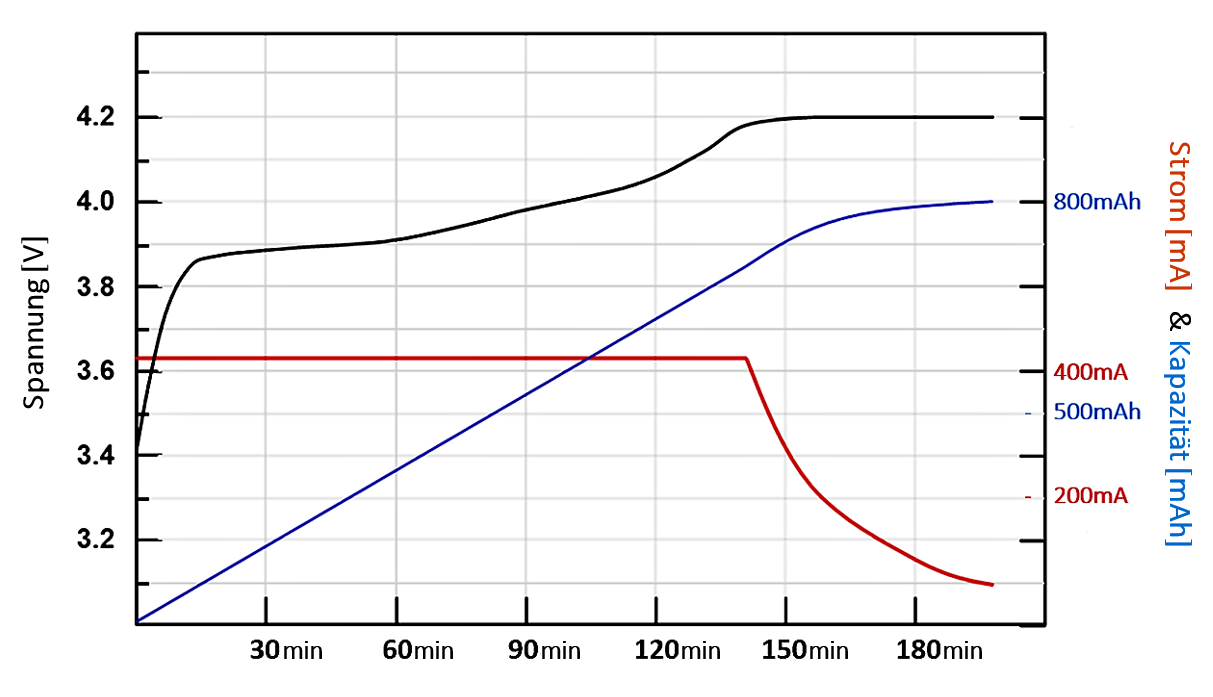
\includegraphics[width=120mm]{data/LadekurveLiIon.png}
		\caption[Blockschaltbild Energiespeicherung]{Blockschaltbild Energiespeicherung} %picture caption
		\label{fig:Ladekurve Li-Ion Akku}
	\end{center}
\end{figure}


Für einen weiteren Schutz, hat die Emmerich LI14500 eine integrierte Schutzbeschaltung namens PCM (Protection Circuit Module). Dieser Schutz garantiert einerseits einen Überladeschutz von 4.25V $\pm$ 0.025V, aber auch einen Tiefentladungsschutz von 2.5V $\pm$ 0.063V. Weiter ist der Akku gegen Überströme ab einer Höhe von 4.8A geschützt und weist zudem einen Schutzschaltungswiderstand von $\leq$ 75mW auf.


\subsection{Ladestation} \label{sec:ladestation}

Nachdem die gesamte induktive Ladeschaltung und Energiespeicherung beschrieben wurde, folgt nun die Beschreibung der Ladestation. Hierfür wurde ein Prototyp erstellt, welche zum einen die gesamte primäre induktive Ladeschaltung beinhaltet. Für den Prototypen wurde eine .stl Datei erstellt, welche mit einem 3D-Drucker gedruckt wurde. Wichtig ist hierbei zu erwähnen, dass es sich nur um einen Prototypen handelt und es bei einer Weiterentwicklung noch Anpassungen geben kann. Da die Ladestation für Versuchszwecke bereits erstellt wurde, ist das Design so gewählt, dass nur ein Dōjō geladen werden kann. Dies könnte in einem weiteren Schritt auf mehrere Ladeaussparungen erweitert werden, wobei mehrere Dōjōs gleichzeitig pro Ladestation geladen werden können. Abbildung \ref{fig:Prototyp} zeigt die Ladestation aus verschiedenen Perspektiven.

\begin{figure}[htbp]
	\centering
	\subfigure[Frontansicht]{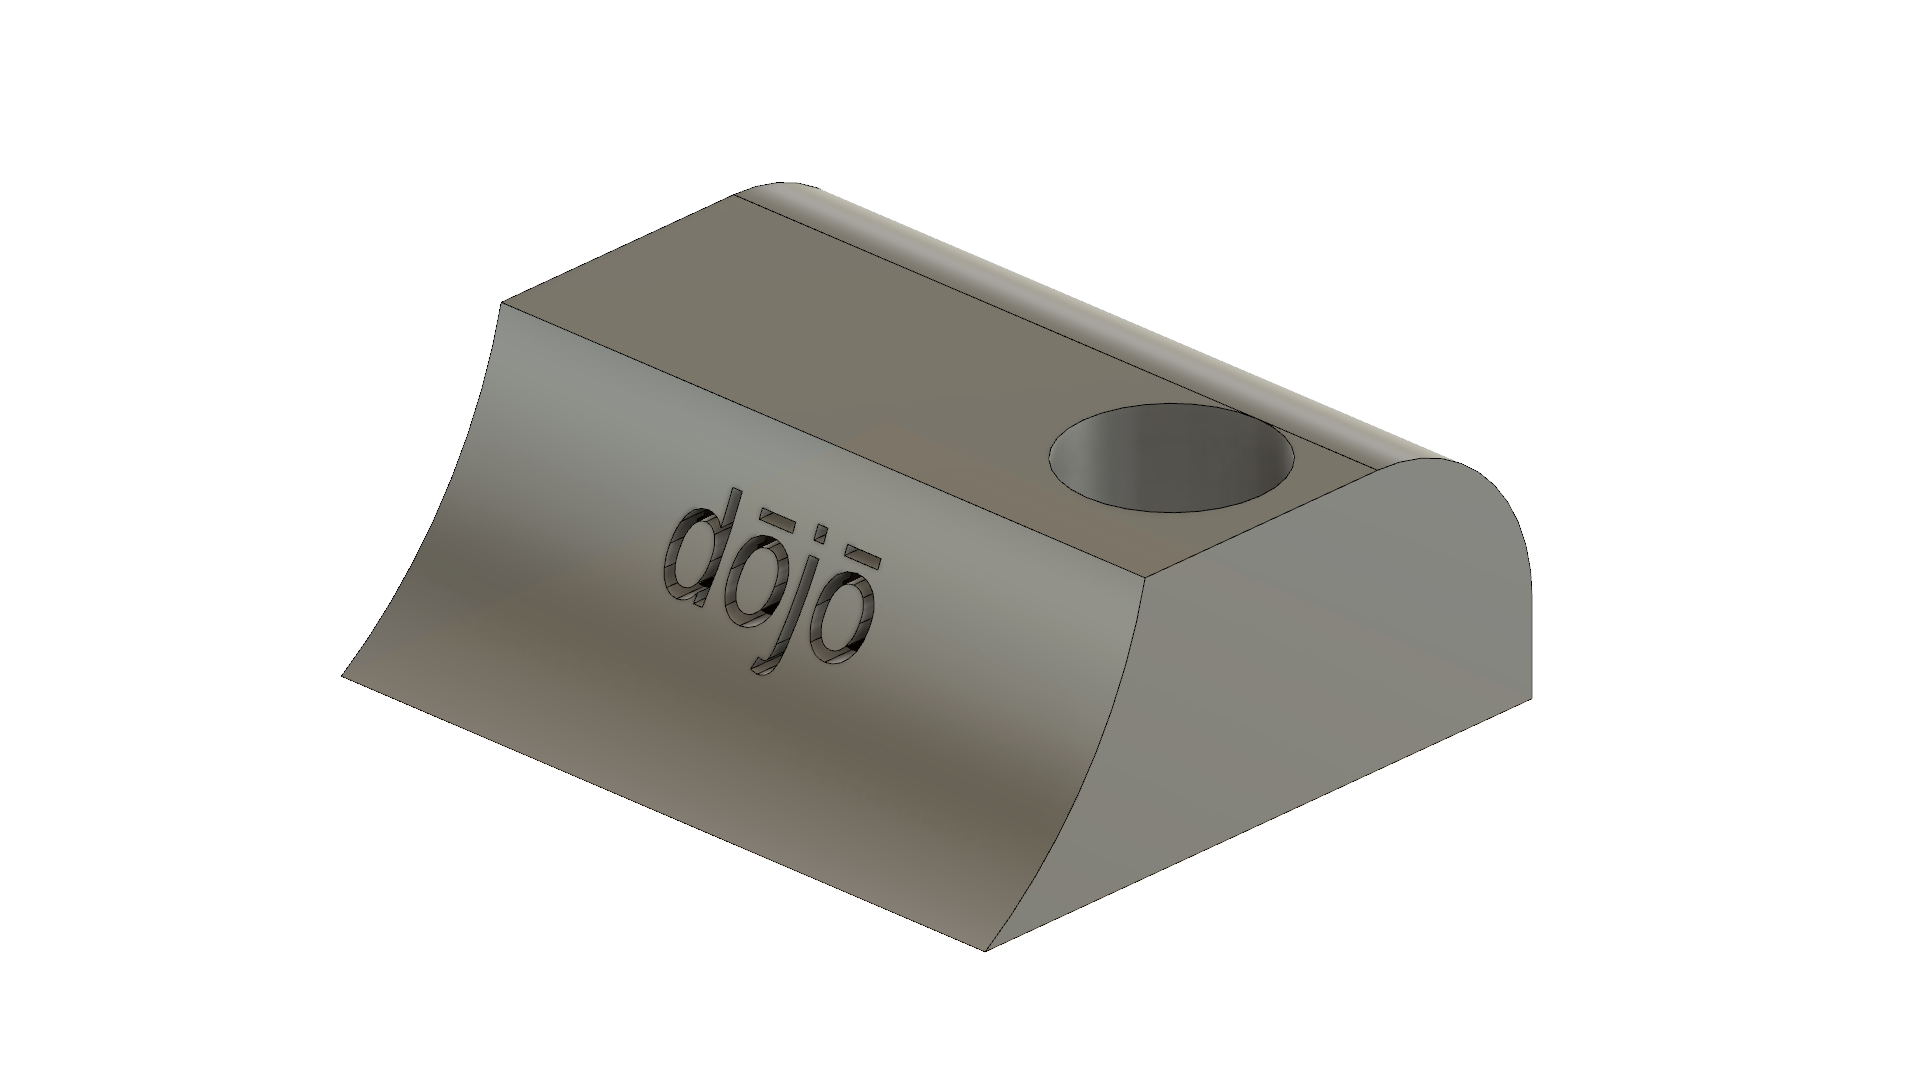
\includegraphics[width = 0.3\textwidth]{data/DojoLadestation01.png}}\quad
	\subfigure[Sicht von oben]{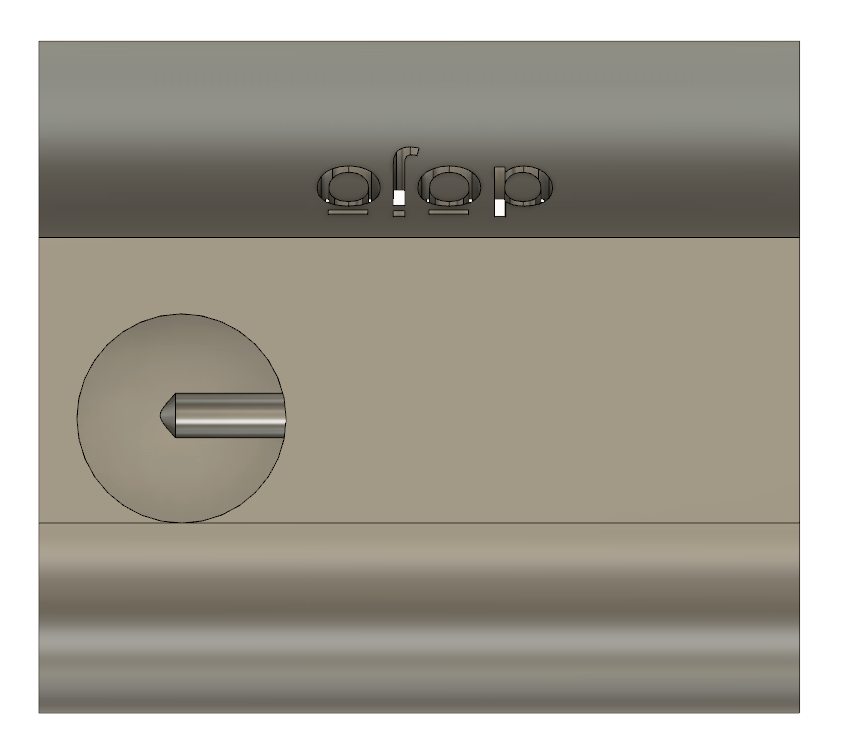
\includegraphics[width = 0.3\textwidth]{data/DojoLadestation02.png}}\quad
	\subfigure[Sicht von unten]{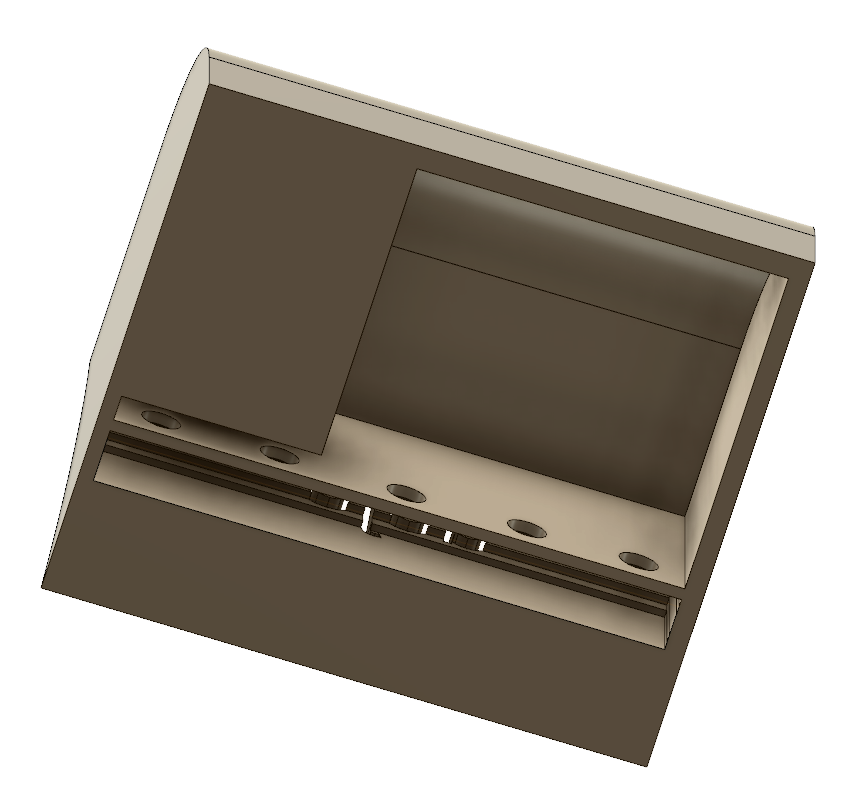
\includegraphics[width = 0.3\textwidth]{data/DojoLadestation03.png}}
	\caption[Prototyp Ladestation]{Prototyp der Ladestation aus verschiedenen Perspektiven}
	\label{fig:Prototyp}
\end{figure}

Die Öffnung dient zum einen als Standhalterung und zum anderen als korrekte Positionierung für die induktive Ladeschaltung. Die richtige Positionierung ist hierbei eines der wichtigsten Kriterien für einen optimalen Ladezyklus, da die Tranceiver- und Receiverspule direkt übereinanderliegend den besten Wirkungsgrad erzielen. Der Hohlraum im Inneren der Ladestation dient zur Platzierung des Primärkreises und hat die Abmessung (80 x 70.7 x 30)mm. Für den Prototypen wurde eine Lochrasterplatine mit allen nötigen Komponenten gefertigt, welche genau in diese Aussparung passt. Weiter sind runde Löcher (5mm $\o$) ersichtlich, welche in die Kammer des Schriftzuges führen. Sie sind für LEDs vorgesehen, welche den Dōjō Schriftzug bei angeschlossener Versorgungsspannung zum Leuchten bringt.
\subsection{Mikrocontroller} \label{sec:microcontrollerHardware}

Als Microcontroller wurde ein nRF52832 der Firma Nordic Semiconductors verwendet, welcher in Abbildung \ref{fig:nRF52832} ersichtlich ist. Seine hohe Performance ermöglicht es ein System aufzubauen, welches den Microcontroller als zentrale Schnittstelle beinhaltet. Der Microcontroller bildet gemäss der Abbildung \ref{fig:Teilsysteme} in Kapitel \ref{sec:gesamtkonzept} bereits beschrieben das Herzstück des Dōjōs. 

\begin{figure}[H]
	\begin{center}
		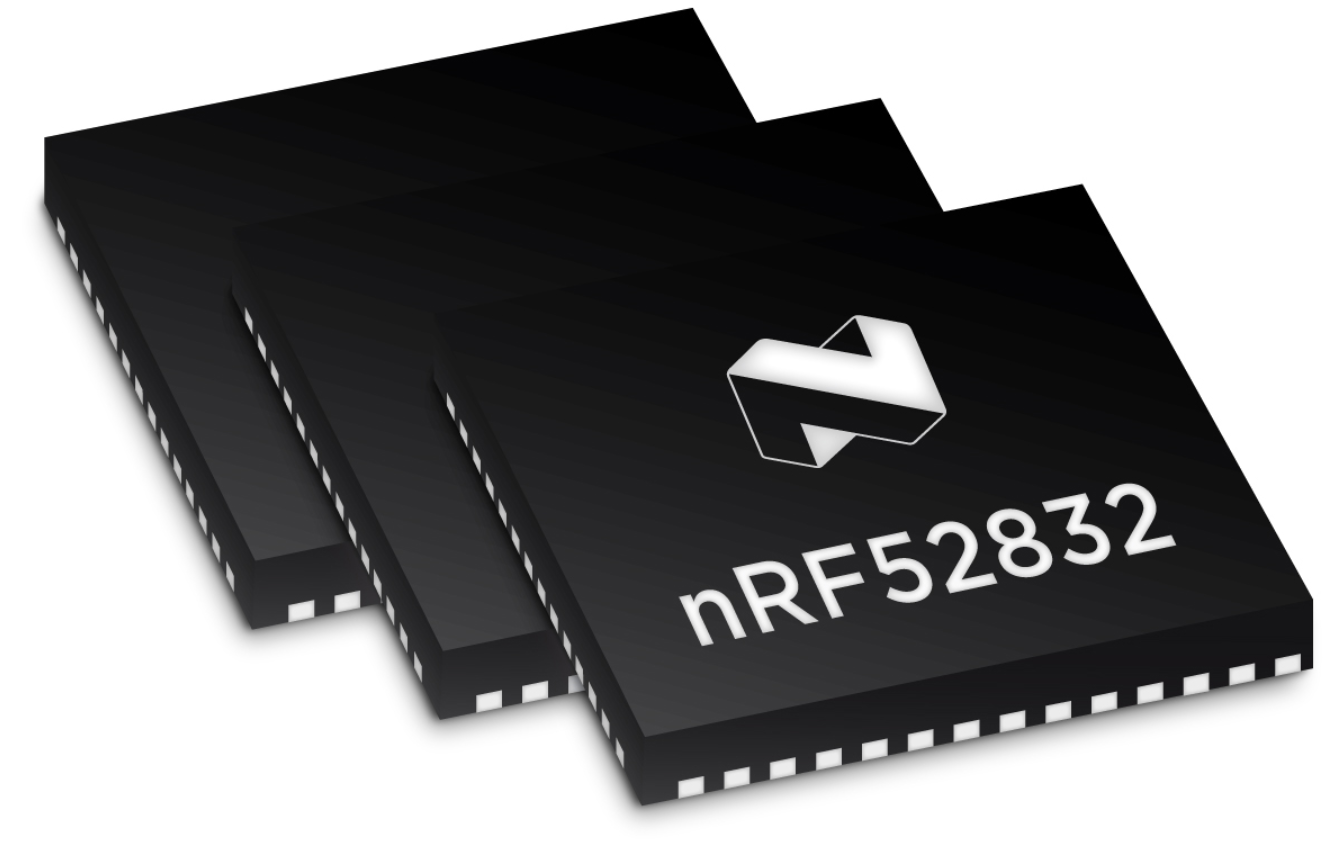
\includegraphics[width=60mm]{data/nRF52832.png}
		\caption[nRF52832 Microcontroller]{nRF52832 Microcontroller \cite{nRF52832}} %picture caption
		\label{fig:nRF52832}
	\end{center}
\end{figure}

Der nRF52832 weist eine Betriebsversorgungsspannung zwischen 1.7V und 3.6V mit einem Versorgungsstrom von 5.4mA auf. Diese niedrigen Werte ermöglichen somit einen dauerhaften Betrieb durch die integrierte Batterie. Die Speicherkapazität ist durch 512kB flash/64kB RAM Speicher gegeben. Für ein einfacheres Handling beim programmieren zu erreichen, wurden für die ersten Tests ein Development Kit (Abbildung \ref{fig:nRF52832-DK}) mit intergriertem nRF52832 verwendet.

\begin{figure}[H]
	\begin{center}
		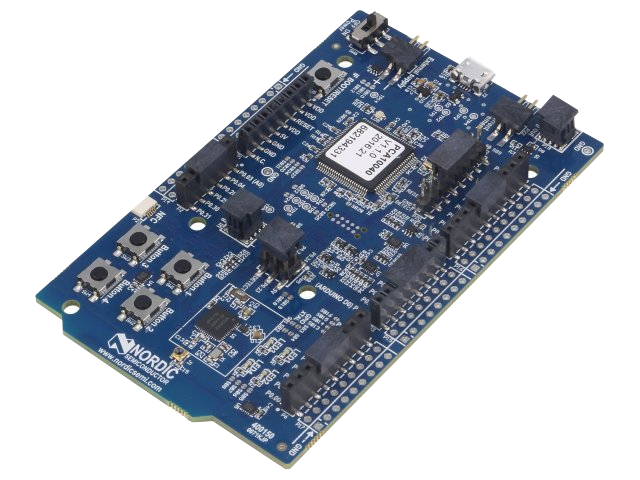
\includegraphics[width=100mm]{data/NRF52-DK.png}
		\caption[nRF52 Development Kit]{nRF52 Development Kit \cite{nRF52-DK}} %picture caption
		\label{fig:nRF52832-DK}
	\end{center}
\end{figure}
 Die Schlüsselmerkmale dieses Boards sind zum einen wie bereits beschrieben der integrierte Microcontroller, zum anderen aber auch eine integrierte Bluetooth Antenne. Das Kit unterstützt zudem proprietäre Bluetooth Smart, ANT und 2.4GHz Applikationen. Es ermöglicht aber auch den Einsatz von Drittanbieter Shields. Dies ermöglicht das Beschreiben und Lesen der SD-Karte zu testen.

\subsection{Filterstufe}\label{sec:filterstufe}
Nachdem die Steuerungseinheit gezeigt wurde, kann nun die Ausgangsstufe erläutert werden. Bevor das Signal verstärkt wird, durchläuft es eine Filterstufe, bestehend aus einer Spule $L$ und einem Kondensator $C$. Das Filter hat die Aufgabe das PWM-Signal des Mikrocontrollers zu filtern und den DC-Anteil zu entfernen. Zusätzlich wird der Mikrocontroller noch vom System entkoppelt. Das wird mit $100\mu F$-Elektrolytkondensatoren an jedem PWM-Ausgang erzielt. Sie werden jeweils seriell geschaltet. Die Dimensionierung der Komponenten wurde mit der nachfolgenden Grundgleichung \ref{eq:LC Filter} durchgeführt:

\begin{equation}
f_g = \frac{1}{2\cdot \pi \cdot \sqrt{L\cdot C}}
\label{eq:LC Filter}
\end{equation}

Nun wird die Grenzfrequenz $f_g$ mit $20 kHz$ festgelegt und ein Kondensator $C$ mit dem Wert $1\mu F$ gewählt. Jetzt kann die Gleichung \ref{eq:LC Filter} nach der Spule $L$ umgestellt werden:

\begin{equation}
L = \frac{1}{(2\cdot \pi \cdot f_g)^2\cdot C }
\label{eq:LC Filter nach L}
\end{equation}

Durch das Einsetzen der Werte für $C$ und $f_g$ in Gleichung \ref{eq:LC Filter nach L} erhält man die folgende Induktivität für die Spule:

\begin{equation}
L = \frac{1}{(2\cdot \pi \cdot f_g)^2\cdot C } = \frac{1}{(2\cdot \pi \cdot 20 kHz)^2\cdot 1 \mu F } = 63.33\mu H
\label{eq:LC Filter nach L 1}
\end{equation}

Unter Einhaltung der {\glqq E12-Reihe\grqq} wird nun der berechnete Wert von $63.33\mu H$ auf den nächstliegenden Wert der Reihe von $68\mu H$ gesetzt. Da es nun zu Abweichungen in der Berechnung kommt, muss die Grenzfrequenz $f_g$ noch mit den bestimmten Bauteilwerten von $L$ und $C$ zurückgerechnet werden. Durch das Einsetzen der Werte in die Gleichung \ref{eq:LC Filter}, erhält man die nachfolgende Grenzfrequenz $f_g$:

\begin{equation}
f_g = \frac{1}{2\cdot \pi \cdot \sqrt{L\cdot C}} = \frac{1}{2\cdot \pi \cdot \sqrt{68\mu H \cdot 1 \mu F}} = 19.3 kHz
\label{eq:LC Filter 1}
\end{equation}

Es ist eine Differenz zur ursprünglichen Annahme von $700 Hz$ zu erkennen, die jedoch in dieser Anwendung vernachlässigt werden kann. In Abbildung \ref{fig:Filterstufe} ist der Aufbau zu sehen. Dabei ist $C_{1}$ der Entkopplungskondensator und $L_{1}$ und $C_{2}$ bilden zusammen die Filterstufe. Rechts ist der Ausgang zur Verstärkerstufe zu sehen, welche im nächsten Kapitel beschrieben wird.


\begin{figure}[H]
	\begin{center}
		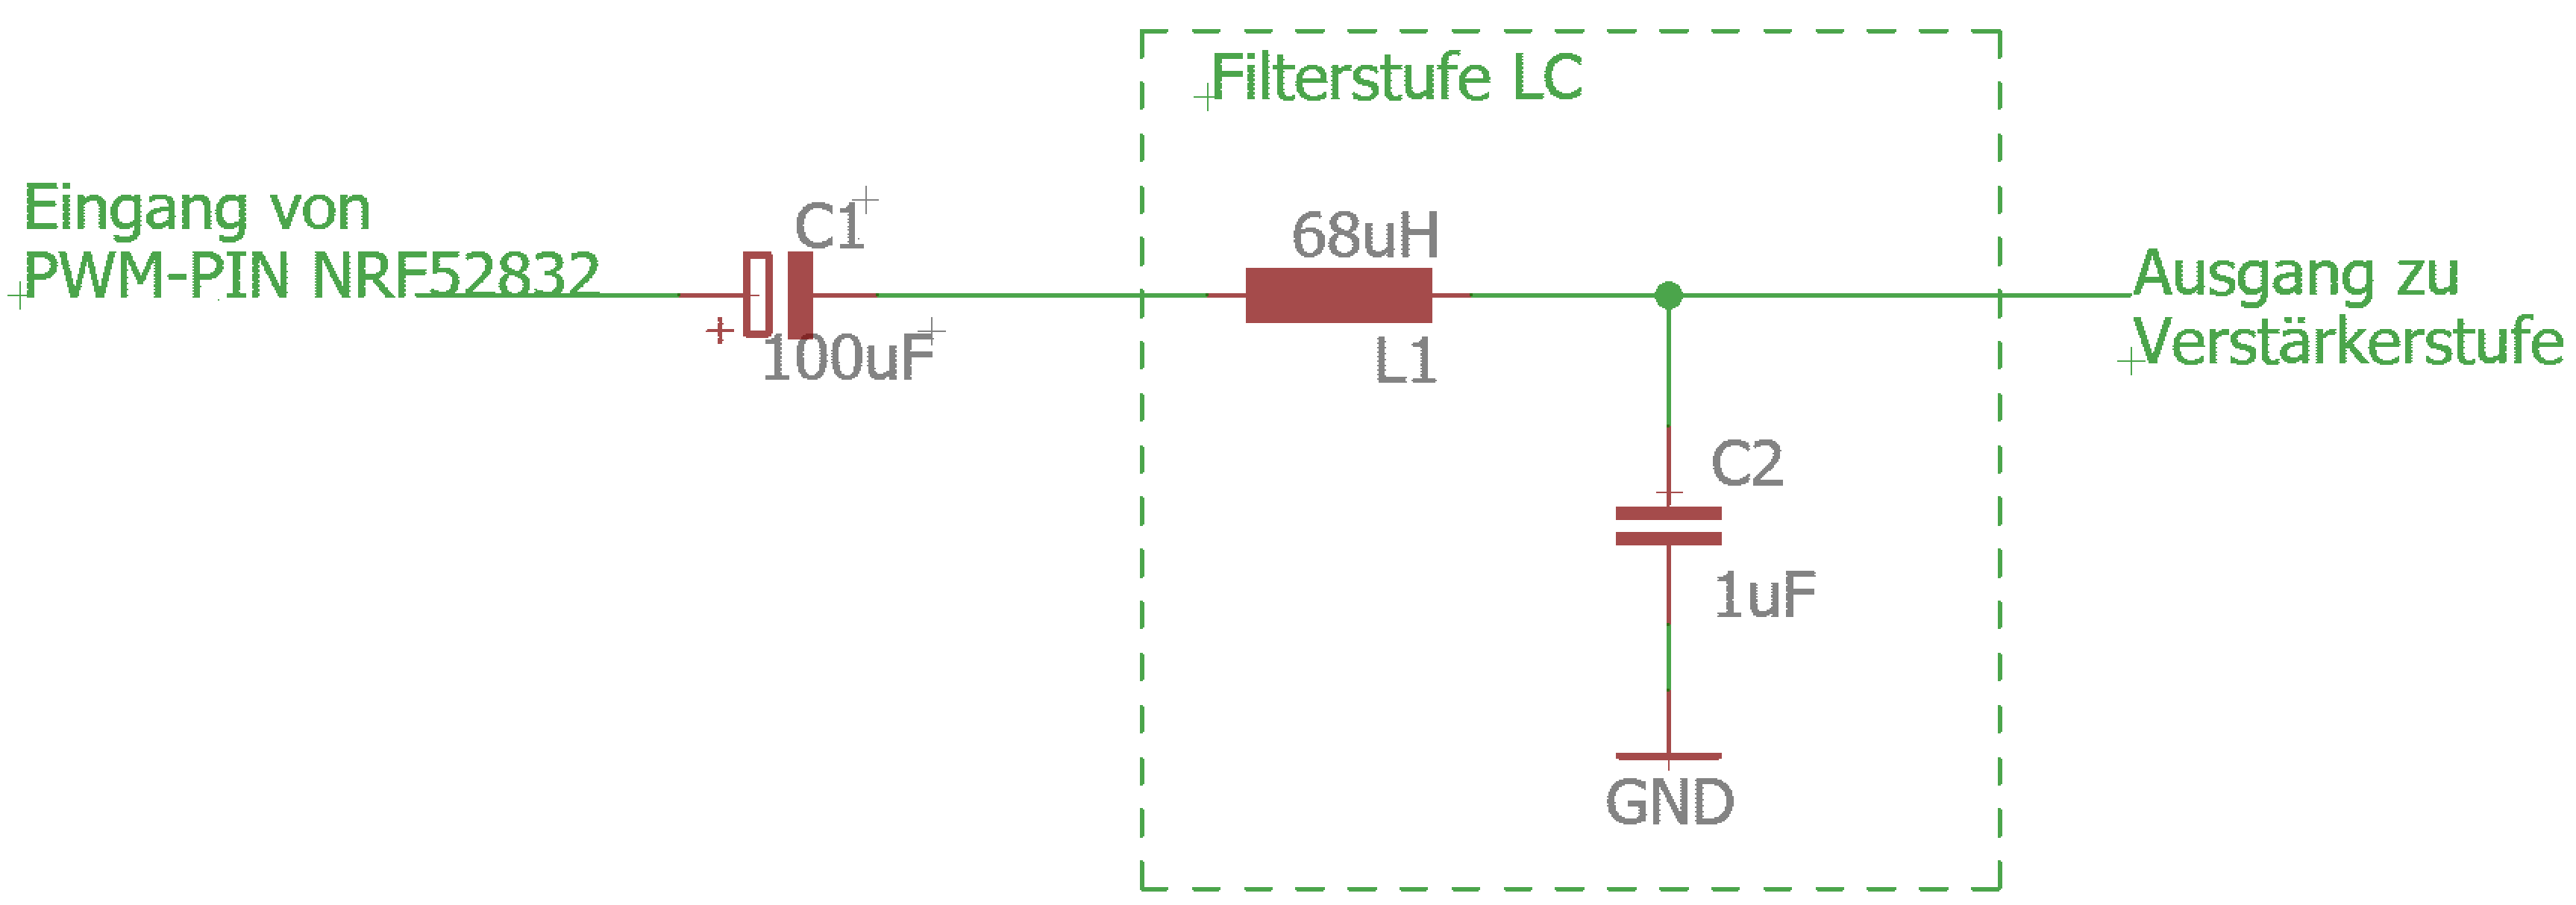
\includegraphics[width=120mm]{data/Schema_Filterstufe.png}
		\caption[Schema der LC-Filterstufe]{Schema der LC-Filterstufe}
		\label{fig:Filterstufe}
	\end{center}
\end{figure}

\subsection{Verstärkerstufe} \label{sec:verstaerkerstufe}
Mit einer Verstärkerstufe lassen sich auf einfache Art und Weise Signale jeglicher Form verstärken. Sie eignen sich bestens, um den Ausgang eines Mikrocontrollers entsprechend aufzubereiten, da die Ausgangsseite meist sehr niedrige Ströme aufweist. Dadurch kann dem Knochenschallaktor genügend Energie zur Verfügung gestellt werden. Prinzipiell gibt es zwei Arten von Verstärkern. Entweder erfolgt die Umsetzung digital oder analog. Beide erfüllen die gleiche Aufgabe, weisen jedoch bezüglich Wirkungsgrad einen deutlichen Unterschied auf. Die digitale Variante weist ungefähr einen Wirkungsgrad von 90$\%$ auf \cite{BoneConductorAdafruit}, während die analoge Variante einen maximalen Wirkungsgrad im Bereich der Leistungsanpassung erzielt \cite{Niklaus_Skript}. Aus diesem Grund wird ein digitaler Verstärker (Class-D-Verstärker) in der Anwendung implementiert. Die Wahl fiel auf den Stereo-Amplifier MAX 98306. Der Verstärker hat in Betrieb einen Stromverbrauch von $143mA$ und eine Speisespannung von $3.3V$. Somit hat er einen Leistungsverbrauch von $471.9 mW$. Im Standby benötigt er lediglich $2 mA$ und somit $6.6 mW$\cite{Verstaerker}. In Abbildung \ref{fig:verstaerkerstufe} ist der schematische Aufbau des Verstärkers dargestellt.

\begin{figure}[H]
	\begin{center}
		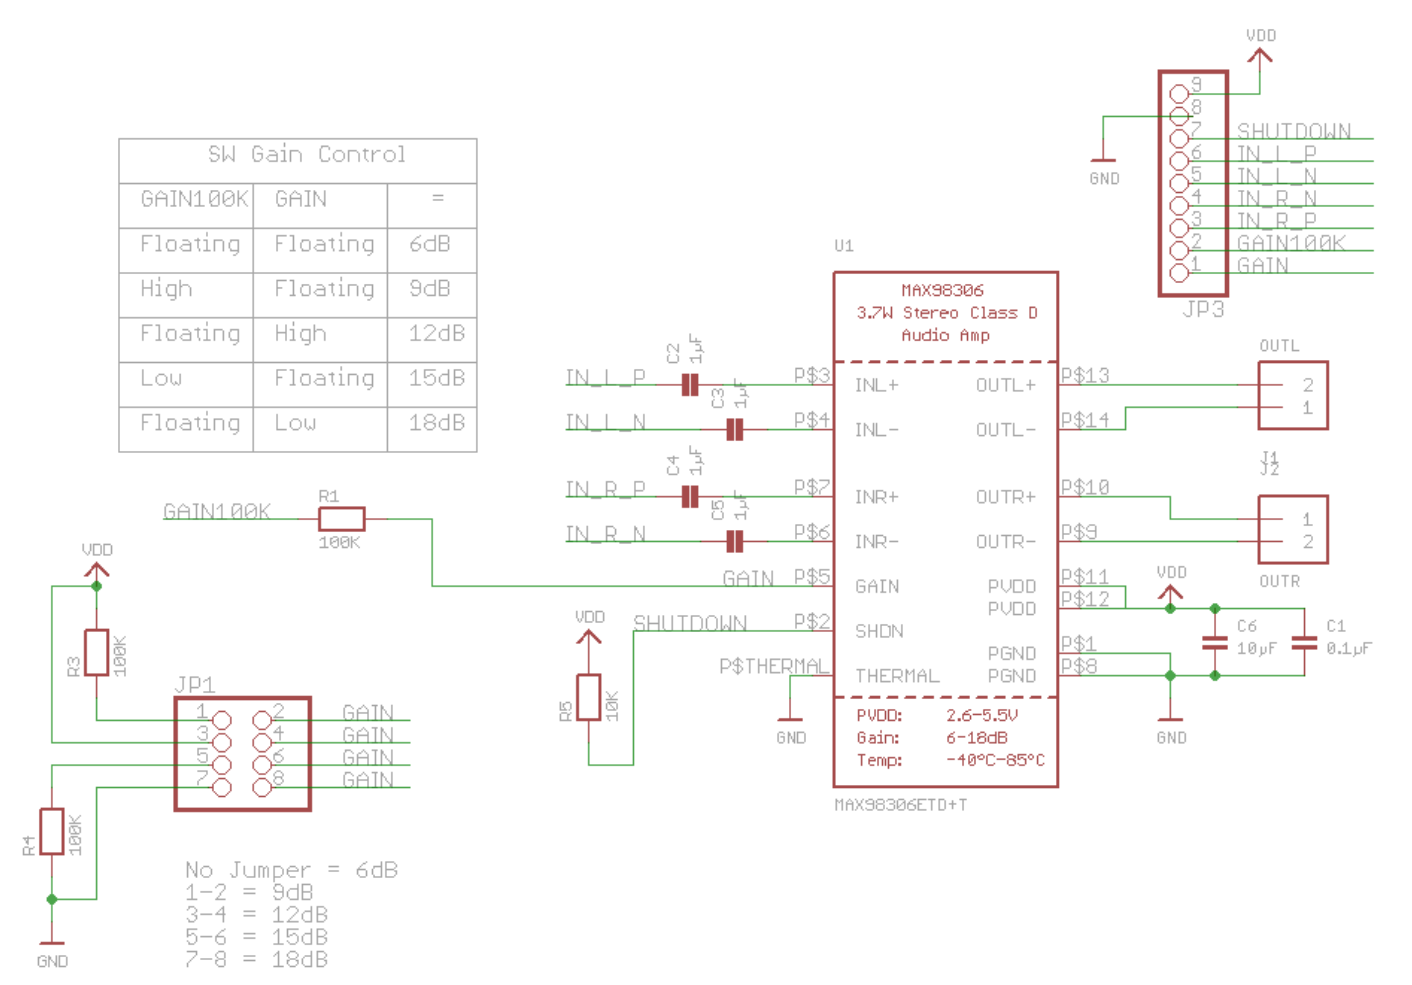
\includegraphics[width=\textwidth]{data/Schema_Verstaerkerstufe.png}
		\caption[Verstärkerstufe \cite{Verstaerker_Schema}]{Schema der Verstärkerstufe} %picture caption
		\label{fig:verstaerkerstufe}
	\end{center}
\end{figure}

\subsection{Knochenschallaktor} \label{sec:knochenschallaktor}
Nachdem das vom Mikrocontroller ausgegebene Audio-File über die Filter- und Verstärkerstufe entsprechend aufbereitet wurde, kann nun die Audiodatei über einen sogenannten Knochenschallaktor ausgegeben werden. Der Aktor arbeitet nach dem Prinzip der Weiterleitung von Schall-Schwingungen oder auch Vibrationen. Dadurch lässt sich der ursprüngliche Gehörgang umgehen und die Schwingungen werden über den Schädelknochen an das Innenohr übertragen. Dies verbessert auch die Hygiene der Anwendung, da kein direkter Kontakt mit dem Gehörgang stattfindet\cite{Knochenschall}. Falls weitere Informationen zur Knochenschalltechnologie gewünscht werden, wird an dieser Stelle auf die Quelle \cite{Knochenschall_HDM_Stuttgart} verwiesen. Für die Anwendung im Dōjō wird ein Knochenschallaktor des Herstellers Adafruit verwendet, welcher in der Abbildung \ref{fig:knochenschallAda} ersichtlich ist.

\begin{figure}[H]
	\begin{center}
		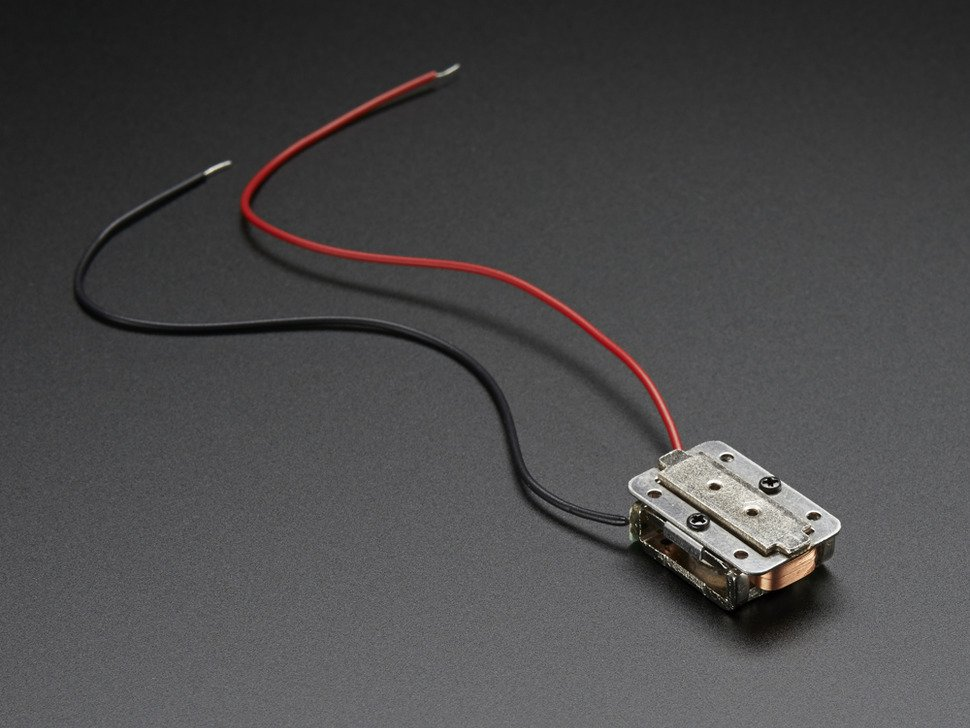
\includegraphics[width=0.6\textwidth]{data/KnochenschallaktorAdafruit1.jpg}
		\caption[Knochenschallaktor \cite{BoneConductorAdafruit}]{Knochenschallaktor von Adafruit} %picture caption
		\label{fig:knochenschallAda}
	\end{center}
\end{figure}

Das ausgewählte Bauteil eignet sich bestens für die Verwendung im Dōjō. Mit einem Gewicht von $9.6 g$ und den Dimensionen $(14\times 21,5\times 7,9) mm$ lässt sich der Aktor gut in das bestehende Gehäuse implementieren \cite{BoneConductorAdafruit}. Weiter ist das Bauteil relativ kostengünstig im Handel erhältlich und kann $1W_{RMS}$ Leistung liefern, was sich dann in der Lautstärke bemerkbar macht. Nach ausführlichen Recherchearbeiten konnten keine wirklichen Alternativen ausgemacht werden. Meist befindet sich die Technologie noch in der Entwicklungsphase oder fällt aufgrund des Preises aus der Auswahlmöglichkeit.

\newpage
\section{Software}\label{sec:software}
%was ich sagen will
%-aufspaltug des Programmes in verschieden Module
%-sdk
%-Nordic
%-Programm typus (Pollend)
%-Viele verweise auf andere Kapitel
%-offene Punkte
%-layer

%Software_Layers.PNG

Es wird ein NRF52832 verwendet von Nordic Semiconductor. Dadurch liegt die Verwendung des Software Development Kit\ref{Nordic SDK} nahe. Dies ist eine Sammlung von Beispielen, Librarys und vorcompilierten Codes. Nachfolgend wird das Software Development Kit nur noch SDK genannt. Es wurde nRF5 SDK v12.3.0 verwendet. Wichtig ist die SDK für ihren integrierten Bluetooth-Stack der verwendet wird. Dieser ist im sogenannten Softdevice enthalten. Um ihn nutzen zu können verwenden wir den S132. Dieser und die nötige Initialisierungen des Bluetooth-Stacks waren in dem Beispielprojekt Uartc in der Central-Rolle vorhanden. Dadurch wurde das ganze Projekt auf diesem Beispiel aufgebaut. Der Softdevice und die SDK legen einige abstraktions Layer auf die Hardware. Diese sind in Abbildung \ref{fig:Software_Layers} visualisiert. Die Die wichtigsten Module des SDK werden im Kapitel \ref{sec:nordicsdk} erklärt, falls weitere Informationen gewünscht sind wird auf die offizielle Dokumentation verwiesen \ref{Nordic.info}.




\subsection{State-Machine}\label{sec:stateMachine}

Nachdem mit dem Einleitungskapitel ein kurzer Überblick geschaffen wurde, kann nun der Hauptteil der Software genauer betrachtet werden. Der gesamte Ablauf basiert auf einer klassischen State-Machine, die aufgrund von unterschiedlichen Parametern in die entsprechenden nächsten States springt. Das hat den Vorteil, dass sich das Programm stets in einem definierten Zustand befindet und mittels entsprechenden Parametern jeweils den nächsten Arbeitsschritt vordefiniert. Die Abbildung \ref{fig:completeStateMachine} zeigt das Gesamtkonzept der State-Machine. Anschliessend werden die einzelnen States genauer definiert und beschrieben.

\begin{figure}[htbp]
	\centering
	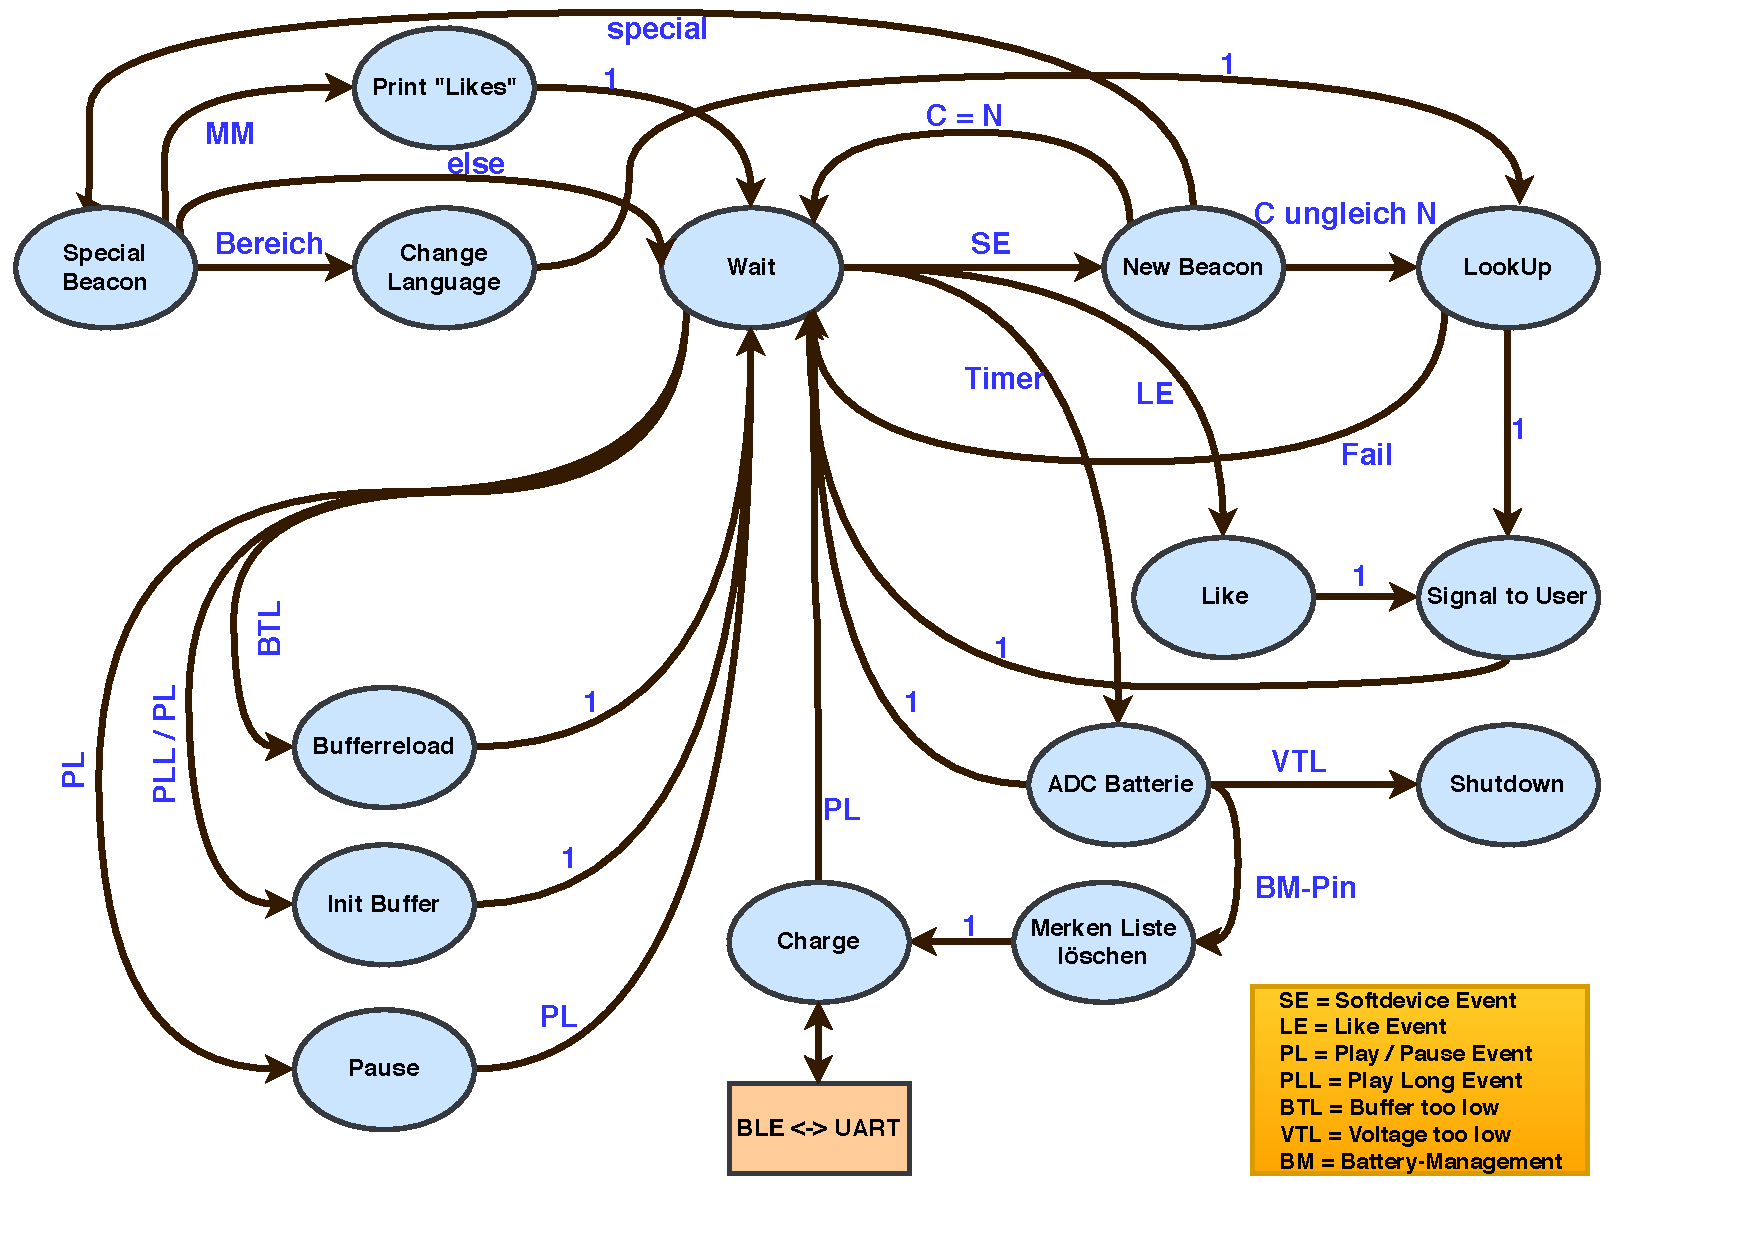
\includegraphics[width=1.15\textwidth]{Data/StateMachineFinal.pdf}
	\caption[Statemachine-Diagramm]{Statemachine im Überblick mit den einzelnen States und den Parametern}
	\label{fig:completeStateMachine}
\end{figure} 

\subsubsection*{State: Lookup}
In diesem State verschafft sich das Programm über die entsprechende Initialisierung Zugriff auf die SD-Karte der Anwendung. Falls der Mikrocontroller nicht auf die SD-Karte zugreifen kann, wird eine Fehlermeldung ausgegeben und die Funktion wird beendet. Anderenfalls wird dem Mikrocontroller signalisiert, dass der Zugriff geglückt ist und die eigentliche Funktion wird gestartet. Dazu werden die beiden Minor- und Majorzahlen in ein hexadezimales Zahlensystem gewandelt, welche dann als Vergleichskriterium verwendet werden. Falls die Nummer gefunden wird, kann das entsprechend zugehörige Audio-File über den Mikrocontroller ausgegeben werden. Verglichen wird jeweils zeilenweise, weshalb auch ein Fehlerhandling eingebaut wurde. Damit wird erkannt, ob sich das Textfile am Ende befindet. Somit lässt sich dann die Suche wiederholen, oder einen Fehler ausgeben. Die nachfolgende Abbildung \ref{fig:lookupState} zeigt den detaillierten Funktionsablauf im Lookup-State.

\begin{figure}[htbp!!!!]
	\centering
	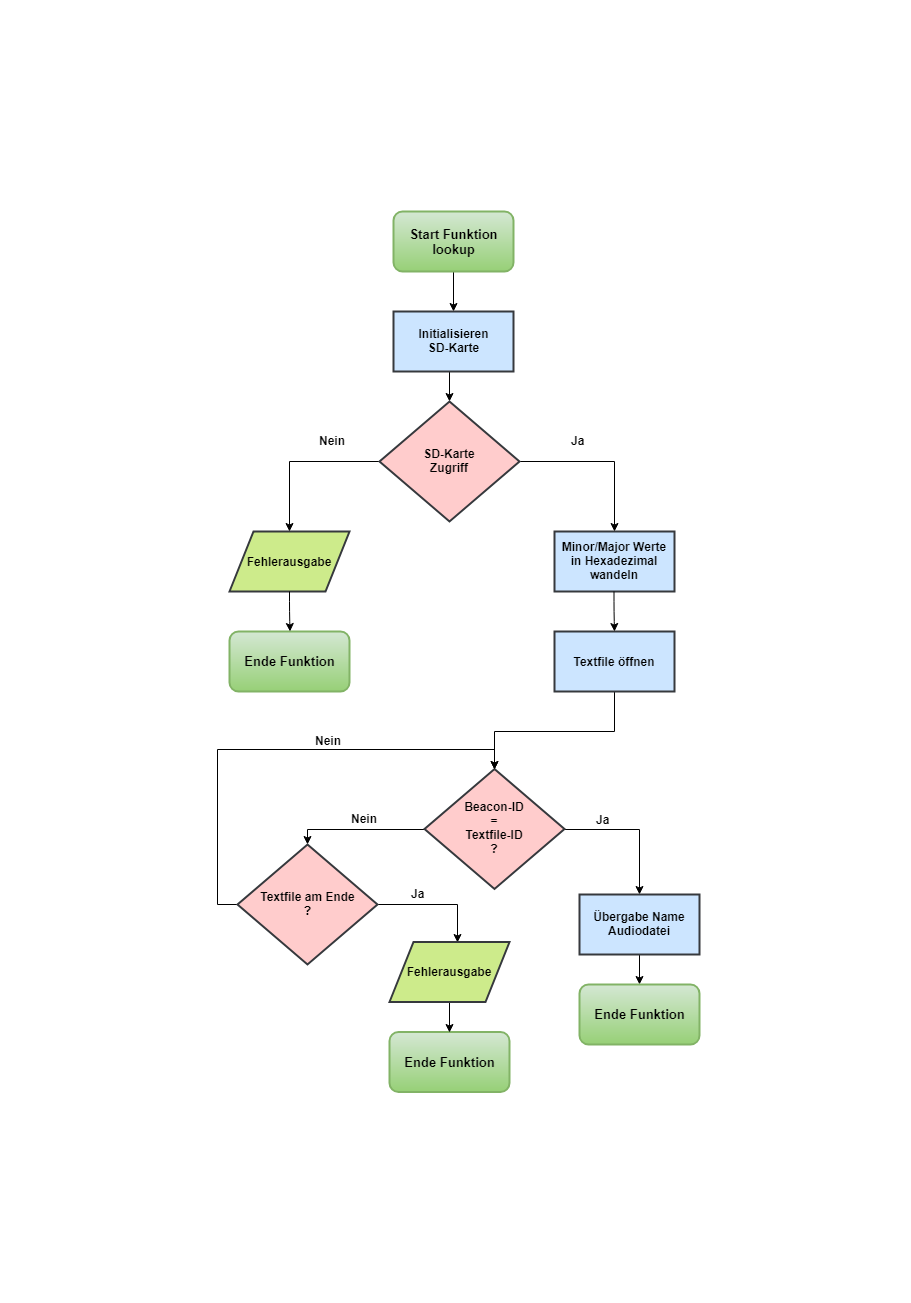
\includegraphics[width=0.57\textwidth]{Data/lookup_picture}
	\caption[Statemachine: lookup]{Funktionsablauf im lookup-State}
	\label{fig:lookupState}
\end{figure} 

\subsubsection*{State: Special Beacon}
Special Beacon dient hauptsächlich zur Unterscheidung der verschiedenen Beacons für die Sprache, das Drucken und weitere Features die in einem weiteren Ansatz implementiert werden können. Aus diesem Grund wurde dieser State auch relativ einfach gehalten. Zuerst wird verglichen, ob es sich dabei um die Sprachkonfiguration handelt. Ist dies zutreffend, so springt das Programm in den Change Language State. Anderenfalls wird überprüft, ob gerade der Like-Button gedrückt wird und entsprechend in den Print \glqq Likes \grqq State gewechselt wird. Ist keine der beiden Zustäde zutreffend, springt das Programm in den Wait State. Die nachfolgende Abbildung \ref{fig:specialBeaconState} zeigt den Ablauf der Funktion.

\begin{figure}[htbp!!!!]
	\centering
	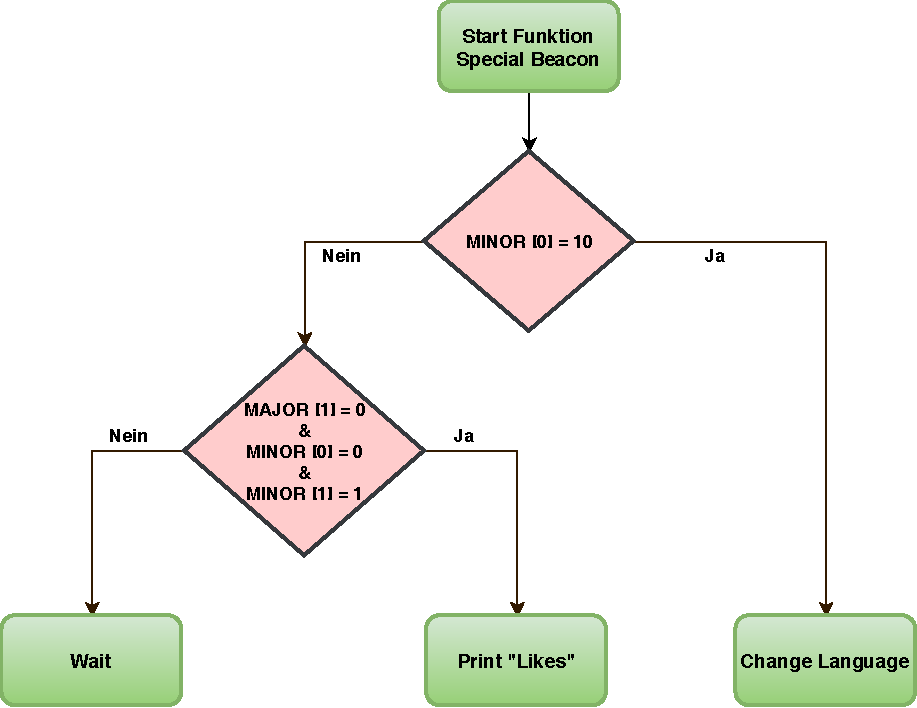
\includegraphics[width=0.9\textwidth]{Data/SpecialBeacon_picture.pdf}
	\caption[Statemachine: Special Beacon]{Funktionsablauf im Special Beacon State}
	\label{fig:specialBeaconState}
\end{figure} 
\newpage
\subsubsection*{State: Change Language}

Dieser State ist für die Sprachauswahl verantwortlich. Aufgrund des Zahlenwertes in Minor [1] wird zwischen den Landessprachen der Schweiz ausgewählt. Dabei wird die Vergleichstabelle in Form einer Datei kopiert und mit einem Kürzel entsprechend der Sprache versehen. Danach springt das Programm wieder in den lookup State.

\begin{figure}[htbp!!!!]
	\centering
	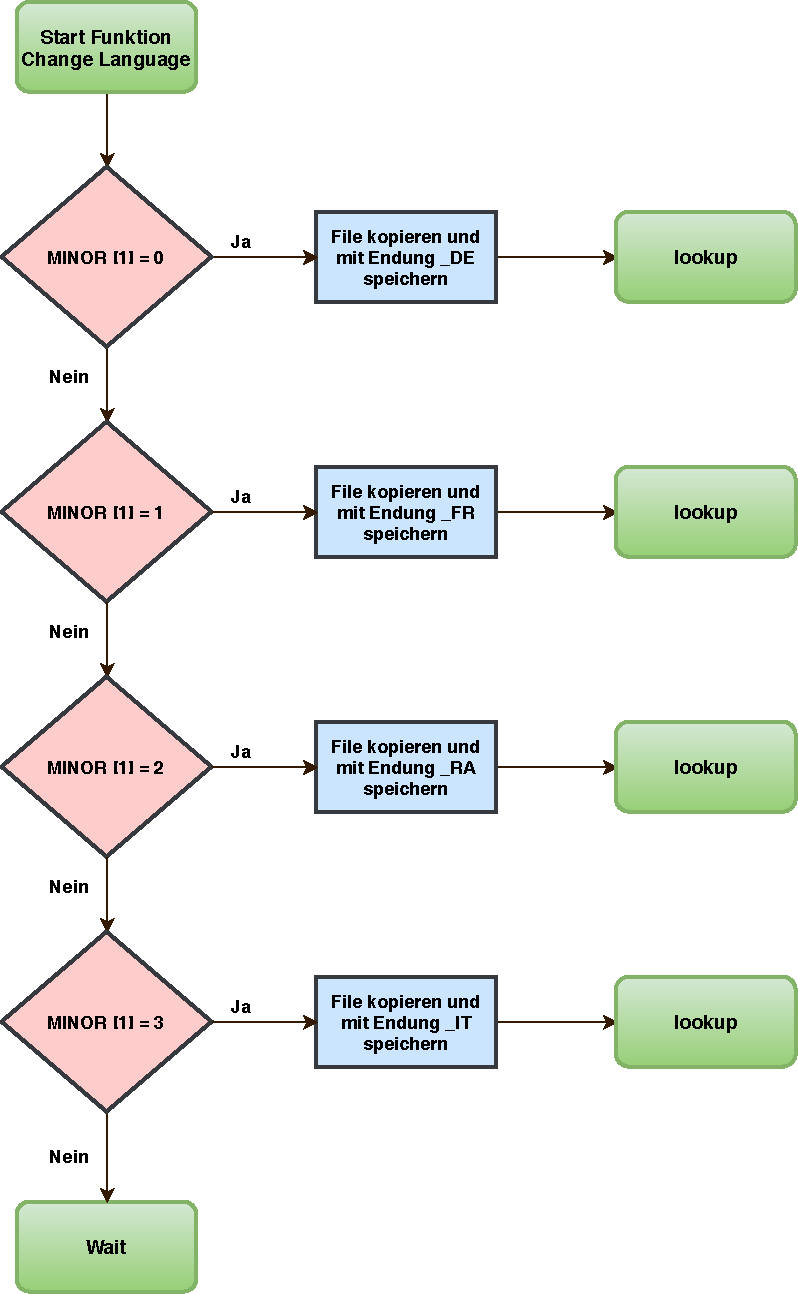
\includegraphics[width=0.7\textwidth]{Data/ChangeLanguage_picture.pdf}
	\caption[Statemachine: Change Language]{Funktionsablauf im Change Language State}
	\label{fig:changeLanguageState}
\end{figure} 

\subsubsection*{State: Print \glqq Likes \grqq}

Print \glqq Likes \grqq wurde nicht implementiert und das Hauptprogramm sprint in den Wait State. Das ist eine optionale Möglichkeit, die in einem weiteren Entwicklungskonzept bearbeitet werden kann. Die Software ermöglicht es aber diese Funktion noch einzubetten. Dabei könnte die Broschüre mit den interessanten Objekten direkt gedruckt werden und bereits für den Besucher am Ausgang des Museums bereit liegen.

\subsubsection*{State: Wait}

[Warte auf Infos Loosli/Elias, noch unklar]

\subsubsection*{State: New Beacon}

In diesem State wird der Ringbuffer ausgelesen. Dadurch lässt sich das Beacon mit dem stärksten Signal identifizieren. Ist das aktuelle Beacon immer noch das gleiche wie das alte Beacon, springt das Programm in den Wait State. Wenn es sich nicht um das gleiche Beacon handelt, wird über den lookup State überprpüft, ob eine entsprechende Übereinstimmung vorhanden ist.

\begin{figure}[htbp!!!!]
	\centering
	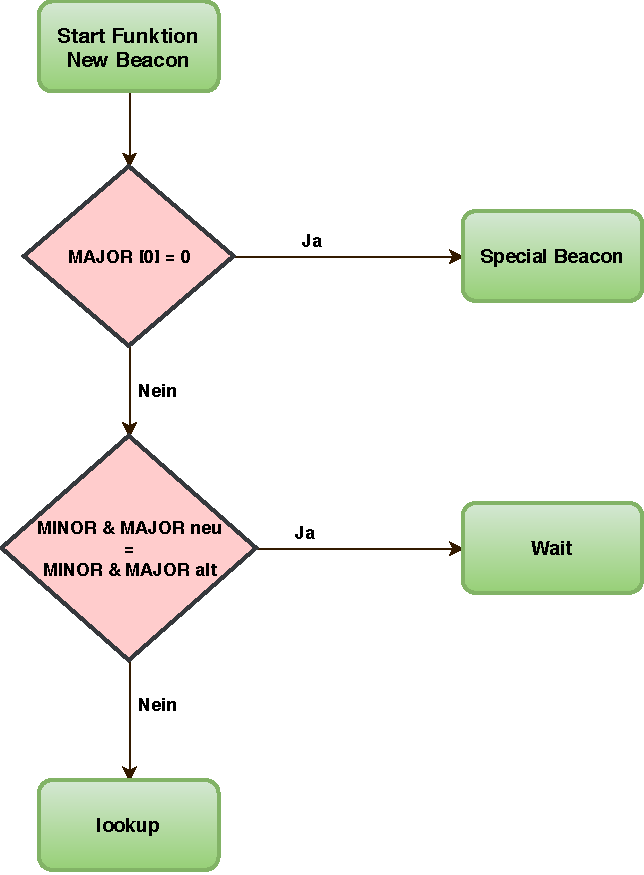
\includegraphics[width=0.5\textwidth]{Data/NewBeacon_picture.pdf}
	\caption[Statemachine: New Beacon]{Funktionsablauf im New Beacon State}
	\label{fig:newBeaconState}
\end{figure} 

\subsubsection*{State: Like}

Wird in diesem State über einen Button ein Like-Ereignis ausgelöst, springt das Programm in den Signal to User State. Findet kein Ereignis statt, dann wird in den Wait State gesprungen.

\begin{figure}[htbp!!!!]
	\centering
	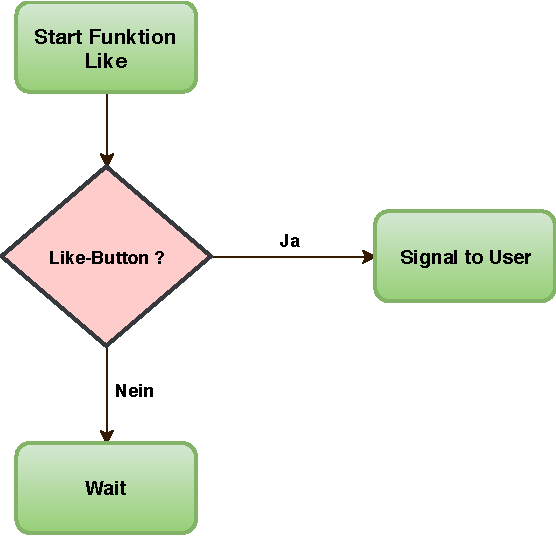
\includegraphics[width=0.5\textwidth]{Data/Like_picture.pdf}
	\caption[Statemachine: Like]{Funktionsablauf im Like State}
	\label{fig:likeState}
\end{figure} 

\subsubsection*{State: Signal to User}

Dieser State hat die Aufgabe, dem Benutzer mitzuteilen, dass ein neues Audio-File verfügbar ist. Dabei blinkt eine dafür vorgesehene LED. Anschliessend springt die Software in den Wait State.

\begin{figure}[htbp!!!!]
	\centering
	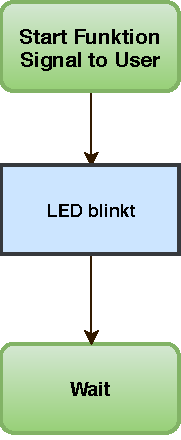
\includegraphics[width=0.2\textwidth]{Data/SignalToUser_picture.pdf}
	\caption[Statemachine: Signal to User]{Funktionsablauf im Signal to User State}
	\label{fig:signalToUserState}
\end{figure} 

\subsubsection*{State: ADC Battery}

[Mehr Informationen benötigt, gemäss Code passiert da gar nichts]

\subsubsection*{State: Shutdown}

[Mehr Informationen benötigt, gemäss Code passiert da gar nichts]

\subsubsection*{State: Merken Liste löschen}

Dieser State löscht die Likes, um für den nächsten User bereit zu sein. Anschliessend folgt der Charge State.

\begin{figure}[htbp!!!!]
	\centering
	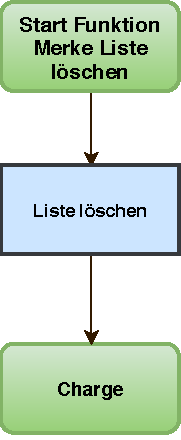
\includegraphics[width=0.2\textwidth]{Data/MerkeListeLoeschen_picture.pdf}
	\caption[Statemachine: Merke Liste löschen]{Funktionsablauf im Merke Liste löschen State}
	\label{fig:merkeListeLoeschenState}
\end{figure} 

\subsubsection*{State: Charge}

[Mehr Informationen benötigt, gemäss Code passiert da gar nichts]

\subsubsection*{State: Pause}

Dieser State pausiert das Sound-File und wartet auf ein weiteres Play-Event, um die Audiodatei wieder abzuspielen.

[Infos von Elias benötigt um das Diagramm zu erstellen]

\subsubsection*{State: Init Buffer}

[Infos von Elias benötigt um das Diagramm zu erstellen]

\subsubsection*{State: Bufferreload}

[Infos von Elias/Loosli benötigt um das Diagramm zu erstellen]
\subsection{Nordic Software Development Kit}\label{sec:nordicsdk}

Das Software Development Kit (SDK) ist eine Sammlung von nützlichem Code für die NRF-Chip Familie. Sie ist sehr umfangreich und ein absolutes Muss für unser Projekt. Hier wird jedoch nur auf ausgewählte Module innerhalb der SDK eingegangen, welche entscheidend sind für das Projekt. Für weitere Informationen wird auf die offizielle Dokumentation \cite{nordic_info} Verwiesen.

\subsubsection*{S132}
Der Softdevice 132 ist ein Protokoll Stack nach Bluetooth 5. Er stellt alle Funktionen des Bluetooth-Low-Energy (BLE) Stacks zur Verfügung, was entscheidend war für das Projekt. Der Stack wird in der Central-Rolle verwendet. Jedoch ist der Softdevice nicht als Code erhältlich, es liegen nur die Binarys bei.

\subsubsection*{Board Support Package (BSP)}
Das Board Support Package ist eine abstraktions Schicht, die das Ziel hat die Hardware von der Software zu trennen und die Portierbarkeit zu erhöhen. Sie arbeitet wie schon der Bluetooth-Stack mit Callbacks. Sie bietet viele Funktionen für typische Hardware, zum Beispiel für Tasten. So kann für kurze und lange Betätigung der Taste ein verschiedenen Callback eingerichtet werden. Die Verlinkung zwischen der Hardware und den entsprechenden Defines findet in File  boards.h statt. Dieses File muss angepasst werden für einen andern Print.

\subsubsection*{NRF Log}
Das Modul NRF Log ist ein mächtiges Debug-Werkzeug. Damit ist es möglich aus der laufenden Software auf eine Konsole zu schreiben. Diese kann frei gewählt werden. Es kann die Segger-Konsole verwendet werden, welche von Nordic empfohlen wird. Das Projektteam verwendete die Variante mit Putty. Weiter können auch Warnungs-Stufen festgelegt werden, was sehr hilfreich ist.

\subsection{Bluetooth}\label{sec:bluetooth}
Ein weiterer wichtiger Baustein der Softwareentwicklung ist das Bluetooth. Aus diesem Grund wird an dieser Stelle das Bluetooth ausführlich behandelt und detailliert erklärt. Gestartet wird mit den Grundlagen. Anschliessend wird das GAP und das GATT beschrieben. Danach folgen die Kapitel BLE-Beacons und RSSI. Am Schluss wird noch die Major- und Minorvergabe behandelt.
\subsubsection{Grundlagen}
Standard-Bluetooth-Geräte senden in einem lizenzfreien Band mit einer Frequenz zwischen 2.402 und 2.480 GHz. Dabei können Störungen durch diverse andere Geräte auftreten, die im selben Frequenzband arbeiten. Um eine Robustheit gegenüber Störungen zu erhalten, wird ein Frequenzsprungverfahren eingesetzt. Dadurch wird das Frequenzband in 79 Kanäle eingeteilt und bis zu 1600-Mal in der Sekunde gewechselt \cite{5_Teildokument_BT}.

Derzeitiger Bluetooth-Standard ist Bluetooth 5. Es zeichnet sich im Gegensatz zu seinen Vorgängern durch eine höhere Reichweite (bis zu 100 m statt 25 m) und eine schnellere Datenrate (bis zu 2 Mbit/s statt 1 Mbit/s) aus. Ausserdem enthält dieser Standard ebenso den im Standard 4 bereits eingeführten {\glqq Low Energy\grqq}-Modus, welcher den schon moderaten Energieverbrauch zusätzlich senkt, was für dieses Projekt sehr wichtig ist \cite{5_Teildokument_BT}. Im Low-Energy-Modus wird das Frequenzband für das Verfahren nicht in 79 sondern in 40 Kanäle unterteilt. Ausserdem wird durch die Datenrate Energie gespart, indem eine Geschwindigkeit von 1 Mbit/s statt 2 Mbit/s erreicht werden kann. Die typische Reichweite im Low-Energy-Modus beträgt 40 m, was die Mindestanforderung von 5 Metern für die Anwendung im Projekt überschreitet und folglich genügt \cite{6_Teildokument_BT}. Damit über Bluetooth Low Energy (BLE) Verbindungen aufgebaut werden können, benötigt es sogenannte Profile. Beim Bluetooth sind dies das GAP (Generic Access Profile) und das GATT (Generic Attribute Profile), auf welche in den nachfolgenden beiden Kapiteln näher eingegangen wird.

\subsubsection{Generic Access Profile}
Das GAP kontrolliert die Verbindungen und die Authentifizierungen. Es beschreibt grundsätzlich die Art und Weise wie Geräte miteinander kommunizieren. Dazu werden zwei verschiedene Rollen für die Geräte definiert. Zum einen die Rolle des zentralen Gerätes und zum anderen die Rolle des Peripheriegerätes \cite{7_Teildokument_BT}. Damit eine Verbindung aufgebaut wird, muss das Peripheriegerät in einem bestimmten Intervall das Payload-Datenpaket senden. Empfängt ein zentrales Gerät das Payload-Paket, kann es für zusätzliche Daten ein Antwortpaket (Scan Response Payload) anfordern, welches daraufhin vom Peripheriegerät gesendet wird \cite{7_Teildokument_BT}. Meistens senden die Peripheriegeräte ihre Authentifizierung und das GATT. Die Authentifizierung dient dem Verbindungsaufbau und das GATT dem grösseren Datentransfer. Solange die Verbindung aktiv ist, kann das Peripheriegerät keine weiteren Verbindungen eingehen. Wird jedoch nur eine kleine Datenmenge benutzt, kann die Datenmenge in das Payload integriert werden, wodurch alle zentralen Geräte in der Nähe einen Zugriff auf die Daten haben. Dieses Verfahren nennt man Broadcasting und ist für dieses Projekt von zentraler Bedeutung. Dennoch wird zuerst im nächsten Kapitel das GATT erläutert \cite{7_Teildokument_BT}.

\subsubsection{Generic Attribute Profile}
Das GATT definiert die Art und Weise, wie Peripherie und zentrales Gerät miteinander Daten austauschen. Dies wird mit Hilfe des Attribute Protocol (ATT) \cite{8_Teildokument_BT} umgesetzt. Das ATT speichert Services, Characteristics und dazugehörende Daten. Services sind logische Sammlungen von zusammengehörenden Characteristics, wobei Characteristics als Datenpunkte betrachtet werden können. Demzufolge besteht das ATT aus einer in Services geordneten Datensammlung \cite{8_Teildokument_BT}. Funktional betrachtet speichern Peripheriegeräte das GATT und dienen somit als GATT-Server. Zentrale Geräte verbinden sich mit Hilfe des GAP mit dem GATT-Server und stellen eine entsprechende Anfrage. Das zentrale Gerät wird somit zum GATT-Client. In einem Intervall werden vom Client gesendete Anfragen vom Server mit Datenpaketen beantwortet. So können grössere Datenpakete ausgetauscht werden, jedoch kein Broadcasting stattfinden \cite{8_Teildokument_BT}. Das genannte zentrale Gerät bzw. GATT-Client ist ind dieser Anwendung der Dōjō. Die genannten Peripheriegeräte sind die BLE-Beacons, welche in der Nähe der jeweiligen Kunstobjekte angebracht sind und im nächsten Kapitel genauer beschrieben werden \cite{8_Teildokument_BT}.

\subsubsection{BLE-Beacons}
BLE-Beacons (Bluetooth Low Energy Beacons) sind kleine Peripheriegeräte, die kleine Informationsmengen übertragen. Wird z.B. ein Temperaturverlauf über ein ganzes Jahr hinweg gemessen, so kommen BLE-Beacons zum Einsatz. Der Grund dafür liegt im Energieverbrauch. Sie können mit einer Knopfzellenbatterie über Jahre hinweg in Betrieb bleiben \cite{9_Teildokument_BT}.

Generell können BLE-Beacons vier Rollen einnehmen, welche in zwei verbindungsfähige Rollen und zwei nicht-verbindungsfähige Rollen eingeteilt werden. Die verbindungsfähigen Rollen sind diejenigen des Peripheriegerätes und des zentralen Gerätes. Die nicht-verbindungsfähigen Rollen sind diejenigen des Senders und des Beobachters. Als Peripheriegerät fungiert das BLE-Beacon als Slave und wartet somit auf einen Input des zentralen Gerätes (Master). Als zentrales Gerät fungiert das BLE-Beacon als Master und kann Verbindungen mit einem oder mehreren anderen Geräten eingehen. Als Sender (Broadcaster) kann das BLE-Beacon zwar keine Verbindngen eingehen, aber vordefinierte Werte senden. Wird das BLE-Beacon als Beobachter (Observer) benutzt, so kann der Observer von einem anderen BLE-Beacon Werte empfangen und an einem angeschlossenen Display anzeigen. Die übermittelten Signale der BLE-Beacons werden gemäss Abbildung \ref{fig:PacketPayload_Header} formatiert \cite{9_Teildokument_BT}.

\begin{figure}[htbp!!!!]
	\begin{center}
		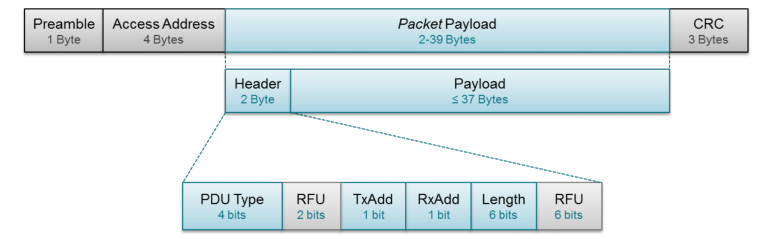
\includegraphics[width=\textwidth]{data/PacketPayload_Header.png}
		\caption[PacketPayload Header \cite{9_Teildokument_BT}]{PacketPayload Header} %picture caption
		\label{fig:PacketPayload_Header}
	\end{center}
\end{figure}

Die Preamble wird zur Synchronisierung und Zeitschätzung benötigt und ist für BLE-Beacons, welche in der Rolle eines Broadcasters sind, immer 0xAA. Auch die Access Address ist für Broadcaster immer gleich, nämlich 0x8E89BED6. Das Payload-Paket beinhaltet Header und Payload. PDU bestimmt den Sendekanaltyp des sendenden Beacons gemäss Tabelle \ref{tab:PDU}.

\begin{table}[htbp!!!]
	\begin{center}
\begin{tabular}{|c|c|c|}
\hline 
\rule[-1ex]{0pt}{2.5ex} PDU Type & Packet Name & Description \\ 
\hline 
\rule[-1ex]{0pt}{2.5ex} 0000 & ADV{\_}IND & Connectable undirected advertising event \\ 
\hline 
\rule[-1ex]{0pt}{2.5ex} 0010 & ADV{\_}NONCONN{\_}IND & Non-connectable undirected advertising event \\ 
\hline 
\rule[-1ex]{0pt}{2.5ex} 0110 & ADV{\_}SCAN{\_}IND & Scannable undirected advertising event \\ 
\hline 
\end{tabular} 
\caption[PDU Type \cite{9_Teildokument_BT}]{PDU Type}
\label{tab:PDU}
\end{center}
\end{table}

RFU (Reserved for Future Use) steht, wie der Name schon sagt, als Reserve für zukünftige weitere Implementationen und wird deshalb derzeit nicht gebraucht. TxAdd definiert, ob die Sendeadresse des Beacons öffentlich (TxAdd = 0) oder zufällig (TxAdd = 1) ist. Das RxAdd tangiert die Beacons nicht und wird deshalb nicht weiter erwähnt. Das CRC (Cyclic Redundancy Check) dient der Erkennung von Fehlübertragungen. Das Payload ist gemäss Abbildung \ref{fig:PacketPayload_Payload} aufgebaut \cite{9_Teildokument_BT}.

\begin{figure}[htbp!!!!]
	\begin{center}
		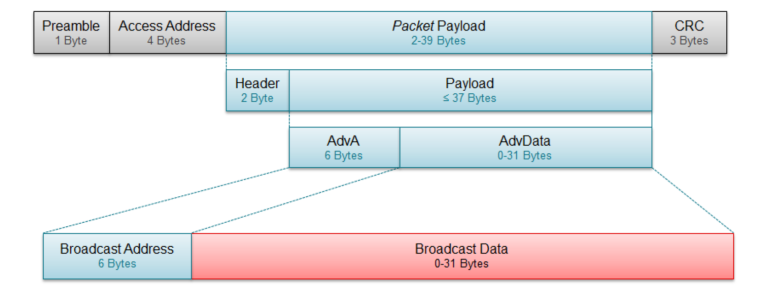
\includegraphics[width=\textwidth]{data/PacketPayload_Payload.png}
		\caption[PacketPayload Payload \cite{9_Teildokument_BT}]{PacketPayload Payload} %picture caption
		\label{fig:PacketPayload_Payload}
	\end{center}
\end{figure}

Es ist zu sehen, dass es mit der Sendeadresse und den Sendedaten gefüllt ist. Die Sendeadresse kann öffentlich oder zufällig sein, wobei eine öffentliche Sendeadresse eine OUI (Organizationally Unique Identifier) nutzt, welche von der IEEE Registration Authority vergeben wird. Die Sendedaten können gemäss der  Tabelle \ref{tab:AD_Data_Type} formatiert werden \cite{9_Teildokument_BT}.

\begin{table}[htbp!!!]
	\begin{center}
\begin{tabular}{|c|c|c|}
\hline 
\rule[-1ex]{0pt}{2.5ex} AD Data Type & Data Type Value & Description \\ 
\hline 
\rule[-1ex]{0pt}{2.5ex} Flags & 0x01 & Device discovery capabilities \\ 
\hline 
\rule[-1ex]{0pt}{2.5ex} Service UUID & 0x02 - 0x07 & Device GATT services \\ 
\hline 
\rule[-1ex]{0pt}{2.5ex} Local Name & 0x08 - 0x09 & Device name \\ 
\hline 
\rule[-1ex]{0pt}{2.5ex} TX Power Level & 0x0A & Device output power \\ 
\hline 
\rule[-1ex]{0pt}{2.5ex} Manufacturer Specific Data & 0xFF & User defined \\ 
\hline 
\end{tabular} 
\caption[AD Data Type \cite{9_Teildokument_BT}]{AD Data Type}
\label{tab:AD_Data_Type}
\end{center}
\end{table}

\begin{table}[htbp!!!]
	\begin{center}
\begin{tabular}{|c|c|c|c|}
\hline 
\rule[-1ex]{0pt}{2.5ex} Byte & Bit & Flag/Value & Description \\ 
\hline 
\rule[-1ex]{0pt}{2.5ex} 0 & • & 0x02 & Length of this data \\ 
\hline 
\rule[-1ex]{0pt}{2.5ex} 1 & • & 0x01 & GAP AD Type Flags \\ 
\hline 
\rule[-1ex]{0pt}{2.5ex} 2 & 0 & LE Limited Discoverable Mode & 180 s advertising \\ 
\hline 
\rule[-1ex]{0pt}{2.5ex} • & 1 & LE General Discoverable Mode & Indefinite advertising time \\ 
\hline 
\rule[-1ex]{0pt}{2.5ex} • & 2 & BR/EDR Not Supported & • \\ 
\hline 
\rule[-1ex]{0pt}{2.5ex} • & 3 & Simultaneous LE and BR/EDR (Controller) & • \\ 
\hline 
\rule[-1ex]{0pt}{2.5ex} • & 4 & Simultaneous LE and BR/EDR (Host) & • \\ 
\hline 
\rule[-1ex]{0pt}{2.5ex} • & 5-7 & • & Reserved \\ 
\hline 
\end{tabular} 
\caption[Flags \cite{9_Teildokument_BT}]{Flags}
\label{tab:Flags}
\end{center}
\end{table}

Die Manufacturer Specific Data können vom Benutzer definiert werden. Hier können Werte gespeichert werden, die das BLE-Beacon senden soll, wie z.B. den RSSI-Wert. Dieser wird im nächsten Kapitel erläutert \cite{9_Teildokument_BT}. Die Flags definieren die Fähigkeiten des BLE-Beacons und sind gemäss der Tabelle \ref{tab:Flags} definiert.

\subsubsection{RSSI}
RSSI steht für Received Signal Strength Indicator und ist ein Indikator für die Empfangsfeldstärke bei der drahtlosen Kommunikation. Je höher dieser Wert ist, desto stärker ist das empfangene Signal \cite{10_Teildokument_BT}. Die drahtlose Kommunikation erfolgt über das Senden von elektromagnetischen Wellen. Trifft eine solche elektromagnetische Welle auf eine Antenne, so führt dies zu einer messbaren Selbstinduktion, welche dem RSSI-Wert entspricht. Dieser Wert muss abhängig von der jeweiligen Anwendung interpretiert werden, da diverse Faktoren bezüglich Transmitter, Receiver und Übertragungsmedium den Wert beeinflussen können.

Im Falle des Museums mit gleichwertigen Beacons bedeutet dies, dass der Besucher sich eher in der Nähe des Beacons mit stärkerem RSSI Wert befindet. Dadurch kann das richtige Audiofile abgespielt werden. Zur Unterscheidung der Beacons werden UUID (Universal Unique Identifier), Major und Minor verwendet. UUID ist im Falle des Projekts eine gewählte Identifikationsnummer für das Museum. Major beschreibt eine eindeutig definierte Zimmernummer und Minor ist die definierte Nummer des Beacons im gleichen Raum. Im nächsten Kapitel wird die Minor- und die Majorvergabe beschrieben.

\subsubsection{Major Minor Vergabe}
Um die Major- und Minornummern mit dem Dōjō zu benutzen, wurden sie im Verlaufe des Projektes standardisiert. Die Sprachauswahl funktioniert über solche Nummern. Beacons mit diesen speziellen Nummern lösen auf dem Dōjō entsprechende Funktionen aus. Abbildung \ref{fig:Bluetooth_def_MM} zeigt die Definitionen. Die Nummernräume sind so gestaltet, dass genug Platz für zusätzliche Funktionen vorhanden ist, wie zum Beispiel für weitere Sprachen oder Zugangskontrollen.

\begin{figure}[htbp!!!!]
	\centering
	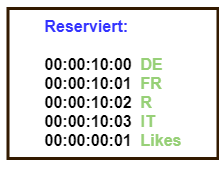
\includegraphics[width=0.35\textwidth]{Data/Reserviert_picture.png}
	\caption[Software:Definierte MM]{Default Definitionen von speziellen Major- und Minornummern.}
	\label{fig:Bluetooth_def_MM}
\end{figure}

In Abbildung \ref{fig:Bluetooth_MM_Vergabe} ist zu sehen, dass die erste Major Nummer 0x00 sein muss, damit ein spezieller Beacon erkannt wird. Das vereinfacht die Software, weil bei einem neuen BLE-Package nur jeweils der erste Eintrag im Array betrachtet werden muss, um die speziellen Beacons zu erkennen. Der Nummernraum für spezielle Beacons umfasst ca. 16 Mio. Adressen, was für zusätzliche Funktionen reichen sollte. Somit bleiben ca. 4.2 Mia. Adressen für Kunstwerke übrig.

\begin{figure}[htbp!!!!]
	\centering
	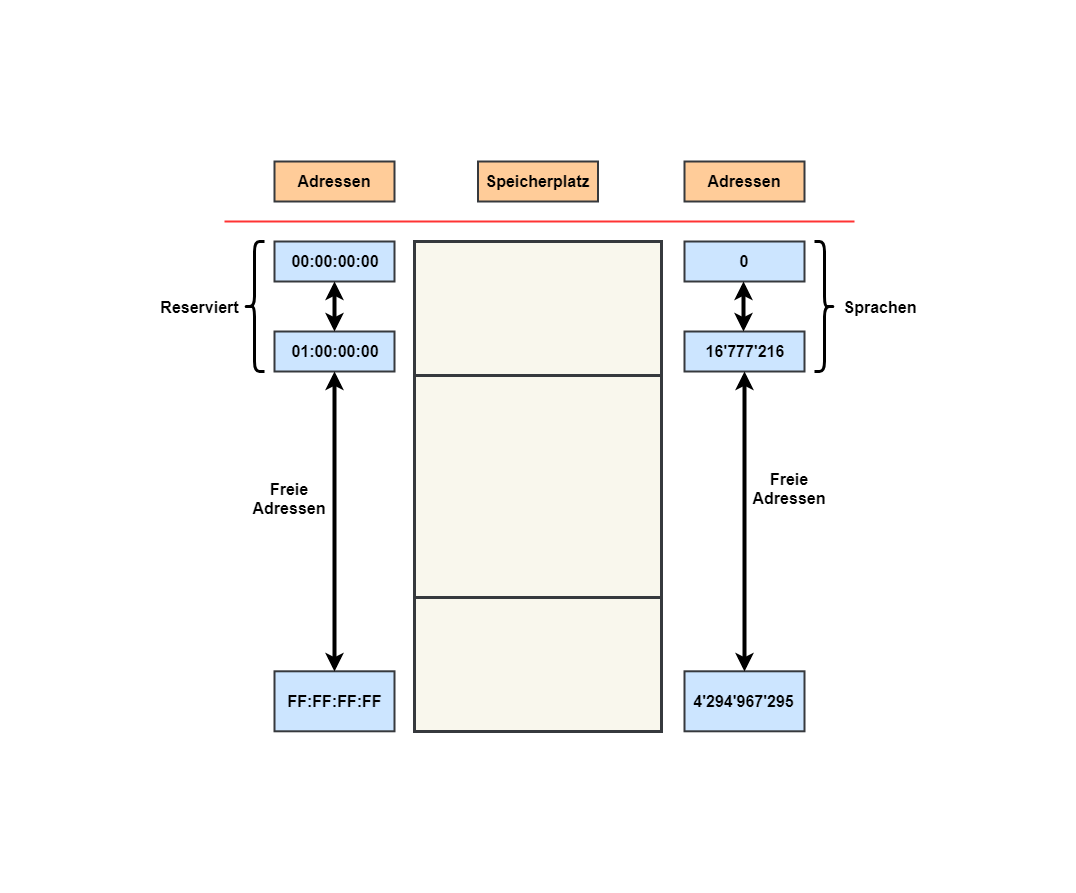
\includegraphics[width=1.0\textwidth]{Data/Speicheradressen_picture}
	\caption[Software:MM Vergabe]{Definition der Majo Minor Vergabe}
	\label{fig:Bluetooth_MM_Vergabe}
\end{figure}



\subsection{SD-Karte}\label{sec:sdKarte}
Um auf die SD-Karte zuzugreifen, wurde die Library fatfs verwendet. Sie ermöglicht einen einfachen Zugriff auf die Daten per SPI-Schnittstelle. Sie wird im ersten Kapitel beschrieben, anschliessend behandelt ein Kapitel die Bündelung des Codes in Zusammenhang mit der SD-Karte, weshalb ein eigenes Modul geschrieben wurde. Der letzte Teil beschreibt noch die benötigten Files auf der SD-Karte, um die Funktionen des Dōjō zu gewährleisten.

\subsubsection{FatFs}
Für den Zugriff auf die SD-Karte wird ein Generic FAT Filesystem Module verwendet. In dieser Library sind Funktionen für die Initialisierung der SD-Karte und den Zugriff auf jene. 

\paragraph{Spezifikationen FatFs}$~~$\\
Dateisystem Typ: FAT, FAT32(rev0.0) und exFAT(rev1.0)\\
Anzahl geöffneter Dateien: unlimitiert (hängt vom verfügbaren Speicher ab)\\
Anzahl Datenträger: bis zu 10\\
Datenträgergrösse: bis zu 2TB bei 512Bytes/Sektor\\
Dateigrösse: bis zu 4GB – 1 auf FAT-Volume und praktisch unbegrenzt auf exFAT-Volume\\
Clustergrösse: Bis zu 128 Sektoren auf FAT-Volume und bis zu 16 MB auf exFAT-Volume	\\
Sektorgrösse:  512, 1024, 2048 und 4096 Bytes[?]\\ 


\subsubsection{SD-Karte Modul}\label{sec:sdKarte modul}
Anschliessend sind die verschiedenen Funktionalitäten aufgelistet.

\subsubsection*{Merken}
Das Modul beinhaltet zwei Funktionen um das Merken zu realisieren. Die Erste speichert das aktuelle Kunstwerk auf eine Liste. Die zweite Funktion löscht eben diese Liste wieder, um den Dōjō für den nächsten Nutzer bereit zu machen. Die Dateinamen der Liste lassen sich im Header-File anpassen.

\subsubsection*{SD-Karte Initialisieren}
Diese Funktion ruft eine Reihe fatfs-Befehle auf, um die SD-Karte zu mounten. Diese wird über ein SPI-Bus an den Mikrocontroller angeschlossen. Die Pins für den Bus lassen sich im Header-File definieren.

\subsubsection*{Lookup}
Diese Funktion ist die eigentliche Implementierung des in Abbildung \ref{fig:lookupState} beschrieben Algorithmus.

\subsubsection*{next\_Value}
Die Funktion next Value dient dazu die nächsten Werte in den Buffer zu laden und ist wie folgt definiert:\\
\textcolor{red}{static void} next\_value(\textcolor{red}{int} bufix)\\
Sie öffnet zuerst die entsprechende Audiodatei. Dies geschieht nur zu Beginn der Datei. Sie bleibt geöffnet bis die Audiodatei zu Ende ist, oder der Benutzer das Abspielen unterbricht. Ebenfalls wird der Lesezeiger beim ersten Aufruf der Funktion auf das $44$ Byte geschoben werden, da die ersten $44$ Bytes eines WAV Files keine Audiodaten enthalten. Die Funktion liest nun 4096 Bytes in einen Hilfsbuffer ein. Die Werte werden dann daraus skaliert und in die Sequenzen geladen. Um die eine invertierte Sequenz zu erzeugen, wird das $15$ Bit auf 1 gesetzt.

\subsubsection*{Sprachwechsel}
Diese Funktion wechselt die Sprache des Dōjō. Die Sprachauswahl geschieht über verschiedene Files. Es exisitert für jede Sprache ein eigenes Lookup-File. Dieses verbindet die Majo-Minor-Kennzeichnungen mit den Wav-Files der jeweiligen Sprache. Dadurch muss für einen Sprachwechsel nur der Zeiger auf das Lookup-File geändert werden.

\subsubsection{Benötigte Files}
Im Header-File des Moduls SD-Karte müssen verschiedene Files definiert werden. Diese müssen auch auf der SD-Karte vorhanden sein und im richtigen Format. Die Merken-Liste ist eine normale .txt Datei. Sie sollte leer sein. Des weiteren müssen die Lookup-Files als CSV (Comma separated Value) Dateien vorhanden sein. Sie sollten dem in Abbildung \ref{fig:definition_lookup_file} definierten Format entsprechen. Zu beachten ist, dass die X Symbole für zwei stellige Hex-Zahlen stehen. Somit hat es eine Referenz auf ein Kunstwerk pro Zeile. Zu beachten ist, dass die Sprachkürzel nur zwei Zeichen beinhalten sollten.

\begin{figure}[H]
	\begin{center}
		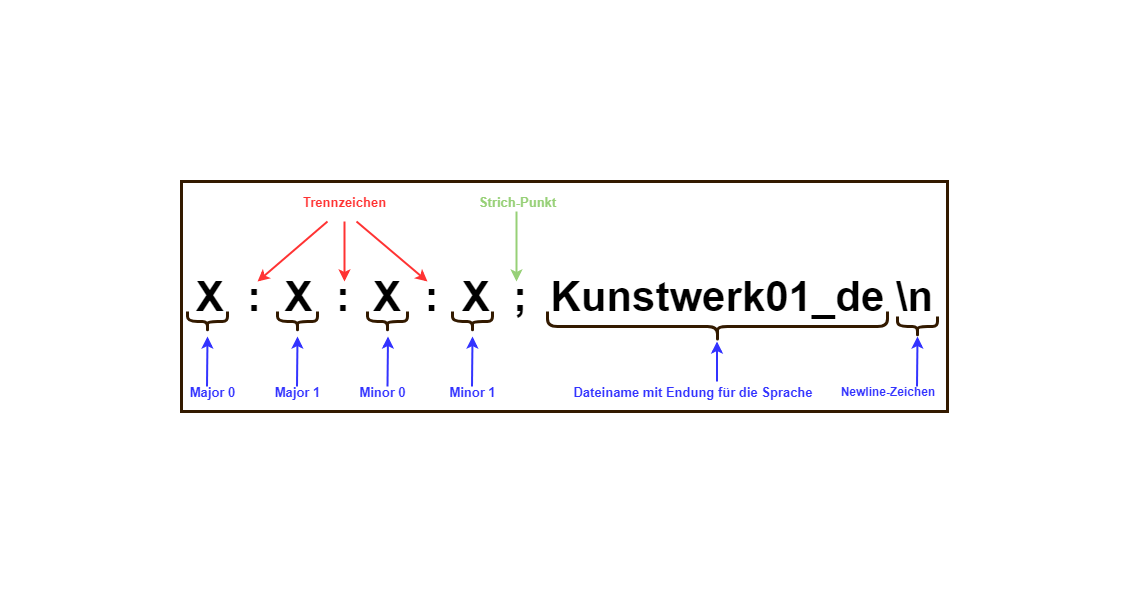
\includegraphics[width=140mm]{data/Definition_picture.png}
		\caption[Formatdefinition Lookup-File]{Formatdefinition Lookup-File} %picture caption
		\label{fig:definition_lookup_file}
	\end{center}
\end{figure}

Die Audiodateien sind im Format WAV Unsigned 8-bit PCM auf der SD-Karte abzulegen. Dabei muss beachtet werden, dass die Sample Frequenz $32 kHz$ beträgt und es sich um eine Mono-Kanal Datei handelt. 

\subsection{Audiowiedergabe durch PWM}\label{sec:audioPWM}
Nachdem der Zugriff und die Kommunikation mit der SD-Karte erklärt wurde, kann an dieser Stelle nun die Audiowiedergabe beschrieben werden. Damit ein Audiosignal abgespielt werden kann, sind zwei PWM-Signale Voraussetzung. Dabei ist das erste Signal das invertierte Signal des zweiten und umgekehrt. Abbildung \ref{fig:pwm_ausgang} zeigt das Prinzip.

\begin{figure}[H]
	\begin{center}
		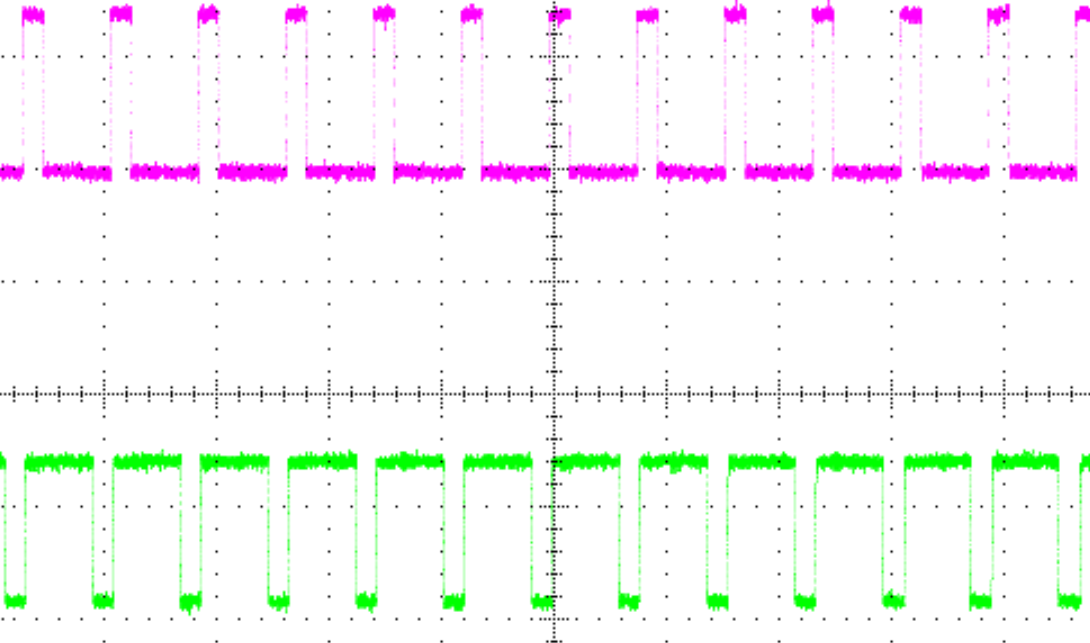
\includegraphics[width=0.7\textwidth]{data/PWM_Signal_500Hz_Mono}
		\caption[PWM-Ausgang des NRF52]{PWM-Ausgang des NRF52: Das violette Signal entspricht dem invertierten grünen Signal} %picture caption
		\label{fig:pwm_ausgang}
	\end{center}
\end{figure}

Das PWM-Signal wird mit dem NRF52-Controller generiert. NORDIC SEMICONDUCTOR stellt dafür die PWM HAL and driver Bibliothek zur Verfügung. Die genutzten Funktionen sind in der Tabelle \ref{table:bibliothek} aufgelistet. Der Controller bietet vier PWM-Instanzen mit je vier Kanälen. Für die Audioausgabe wurden zwei PWM-Instanzen mit je einem Kanal genutzt.

\begin{table}[H]
	\begin{center}
	\begin{tabular}{|l|l|l|}
		\hline
		%\rowcolor[HTML]{C0C0C0} 
		\textbf{Beschreibung} & \textbf{Funktion}                & \textbf{Argumente}                                                                                                                                                                                                            \\ \hline
		PWM initialisiern     & nrf\_drv\_pwm\_init              & \begin{tabular}[c]{@{}l@{}}nrf\_drv\_pwm\_t const *const p\_instance\\ nrf\_drv\_pwm\_config\_tconst *p\_config\\ nrf\_drv\_pwm\_handler\_thandler\end{tabular}                                                               \\ \hline
		Audio abspielen         & nrf\_drv\_pwm\_complex\_playback & \begin{tabular}[c]{@{}l@{}}nrf\_drv\_pwm\_t const *const p\_instance\\ nrf\_pwm\_sequence\_t const *p\_sequence\_0\\ nrf\_pwm\_sequence\_tconst *p\_sequence\_1\\ uint16\_t  playback\_count \\ uint32\_t  flags\end{tabular} \\ \hline
	\end{tabular}
	\caption[Funktionen der PWM HAL and driver Bibliothek]{Funktionen der PWM HAL and driver Bibliothek}
	\label{table:bibliothek}
\end{center}
\end{table}

Abbildung \ref{fig:pwm_ablauf} zeigt den Ablauf des PWM-Unterprogramms. Zuerst findet die Initialisierung statt. Anschliessend können die beiden Sequenzen 0 und 1 generiert werden, in welchen die Daten des Audio-Files abgelegt werden. Die Funktion complex\_playback generiert dann aufgrund der Sequenzen das entsprechende PWM-Signal am Ausgang. Nachfolgend werden die einzelnen Schritte noch detaillierter beschrieben.

\begin{figure}[H]
	\begin{center}
		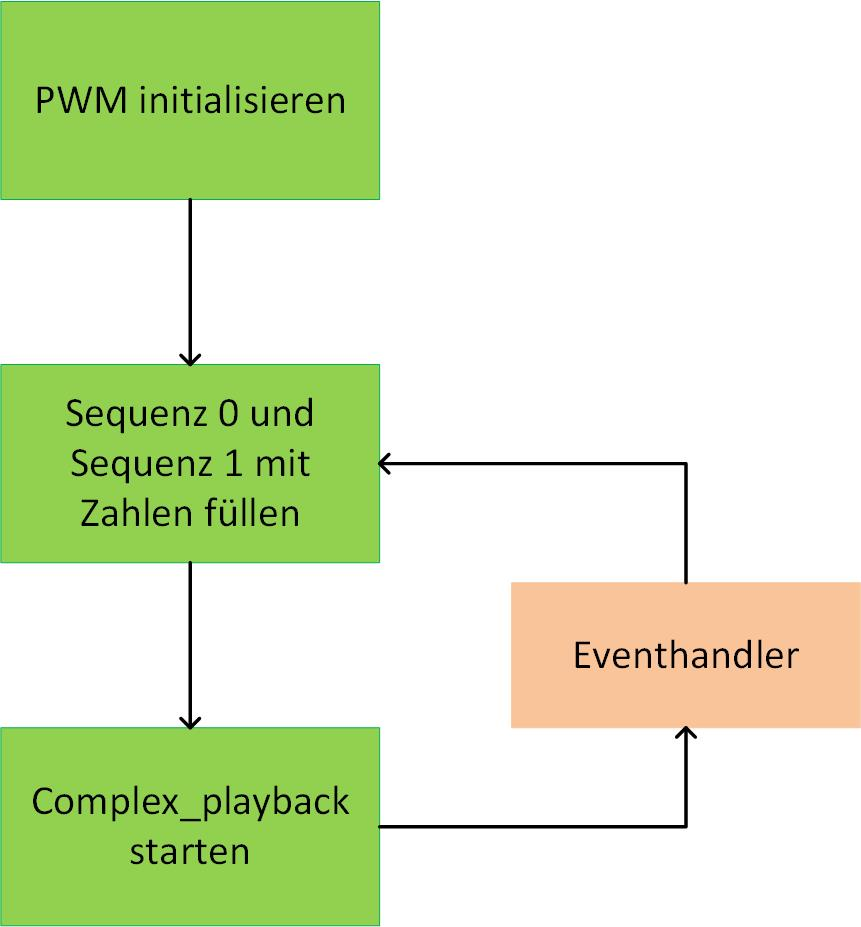
\includegraphics[width=0.5\textwidth]{data/pwm_ablauf}
		\caption[Ablauf PWM-Ausgabe]{Ablauf PWM-Ausgabe} %picture caption
		\label{fig:pwm_ablauf}
	\end{center}
\end{figure}

\subsubsection*{PWM Initialisieren}\label{sec:PWM initialisieren}
Bei der PWM-Initialisierung wurde die PWM-Instanz, die Config und der Eventhandler mitgegeben. Die Config des PWM musste anhand der Angaben des Wavefiles generiert werden. Die Werte wurden gemäss Tabelle \ref{table:config} gewählt.

\begin{table}[H]
	\centering
	\begin{tabular}{|l|l|l|}
	\hline
	\textbf{Parameter}  & \textbf{Gewählter Wert}    & \textbf{Bemerkung}                                                           \\ \hline
	output\_pins  & Pin 17                        & \begin{tabular}[c]{@{}l@{}} Pin 17 für PWM Modul 1                                                        \\ Pin 27 für PWM Modul 2 \end{tabular} 
	 \\ \hline
	irq\_priority & APP\_IRQ\_PRIORITY\_LOWEST & \begin{tabular}[c]{@{}l@{}} Wurde so gewählt, da keine \\ 	 anderen Interruptroutinen vorhanden \end{tabular} 
	 \\ \hline
	base\_clock   & NRF\_PWM\_CLK\_16MHz       & Es wurde die maximale clock Frequenz gewählt                                  \\ \hline
	count\_mode   & NRF\_PWM\_MODE\_UP         & PWM zählt bis zu top\_value
	 \\ \hline
	top\_value    & 500                        & Siehe Berechnung top\_value                                                            \\ \hline
	load\_mode    & NRF\_PWM\_LOAD\_COMMON     & \begin{tabular}[c]{@{}l@{}}Wurde gewählt, da alle PWM Kanäle \\ den selben Wert ausgeben\end{tabular} \\ \hline
	stepp\_mode   & NRF\_PWM\_STEP\_AUTO       &\begin{tabular}[c]{@{}l@{}} Jedes Sample wird gemäss der Anzahl \\ 	 definierter Wiederholungen abgespielt \end{tabular} 
	 \\ \hline
	\end{tabular}
	\caption{Gewählte Config Werte}
	\label{table:config}
\end{table}

\textbf{Berechnung top\_value}\\
Da die clock Frequenz (in Tabelle \ref{table:config}  base\_clock) des PWM Moduls auf $16MHz$ gesetzt wurde, beträgt der top\_value für eine Audiodatei mit Abtastfrequenz von $32kHz \;  500$. Dies berechnet sich wie folgt:
\begin{equation}
32kHz = \frac{16MHz}{top\_value}
 \Rightarrow \; top\_value = \frac{16MHz}{32kHz} = 500
\end{equation}

\subsubsection*{Sequenzen laden}\label{sec:Sequenzen befüllen}
Jetzt können die Sequenzen geladen werden. Mit der Funktion next\_Value werden neue Werte in die entsprechenden Sequenzen geladen. Diese Funktion ist im Kapitel \ref{sec:sdKarte} genauer beschrieben.

\subsubsection*{Complex playback}\label{sec:Complex playback}
Die Funktion generiert anhand der Sequenz ein entsprechendes PWM-Signal. Der
Vorteil zu simple playback ist, dass zwei Sequenzen mitgegeben werden können. Wenn die Sequenz 0 fertig abgespielt wurde, startet automatisch die zweite Sequenz und der Eventhandler wird ausgelöst. In dieser Zeit kann die erste Sequenz wieder neu beladen werden. Die Beladung der Sequenzen wird mit dem Eventhandler dieser Funktion gesteuert. 

\subsection{Lizenzen}\label{sec:lizenzen}
Die Lizenztexte sind alle in Englisch veröffentlicht. Dadurch kann das Projektteam nicht haftbar gemacht werden für unwissentlich gemachte Übersetzungsfehler.

\subsubsection*{SDK}
Nordic Semiconductor hat an Anfang eines jeden Files ihren Lizenztext \cite{nordic_sdk_license} hinterlegt. In diesem ist Beschrieben was mit dem Code gemacht werden darf und was nicht. Einige wichtige Punkte:

\begin{itemize}
	\item Am Anfang jedes Files muss der Lizenztext stehen.
	\item Weiterverteilung muss unter dem Selben Copyright erfolgen wie bisher.
	\item Mann soll nicht ungefragt Werbung machen für Nordic und Co.
	\item Die Software darf nur für NRF-Chips verwendet werden.
\end{itemize}

Auch werden alle Verantwortungen für Support, Sicherheit usw. abgestritten. Damit sind sie nicht Haftbar für Schäden, die die Software anrichtet.

Der S132 ist speziell, weil dieser nicht in Source-Form vorliegt. Er ist nur in Binary-Form enthalten. Er hat einen leicht anderen Lizenztext welcher in der SDK neben den Biarys gefunden werden kann. Er besagt zusätzlich, dass der Sourcecode der Softdevice nicht reverse engineered, decompilert, modifiziert und disassembliert werden darf.

\newpage
\section{Validierung} \label{sec:validierung}

Bei der Validierung werden nachfolgend die Testkonzepte der Hardware und der Software erläutert. Die Hardware beinhaltet hierbei hauptsächlich das Testen der Batterie, der induktiven Ladeschaltung und der Filterstufe. Danach folgt das Testkonzept der Software. Es beinhaltet das Testen des PWM-Signals, der Statemachine, des Bluetooths und zum Schluss noch das Testen der SD-Karte.
\subsection{Testkonzept Hardware}\label{sec:testkonzeptHardware}
Damit ein reibungsloser Betrieb möglich ist, müssen die einzelnen Hardware Komponenten auf Herz und Nieren geprüft werden. Nachfolgend werden die Testverfahren genauer beschrieben und die Testergebnisse aufgelistet.

\subsubsection*{Schutzmechanismen Batterie}\label{sec:batterie}
Die Batterie weist einige Schutzmechanismen auf, welche alle getestet werden müssen. Als erstes wurde der Tiefentladungsschutz geprüft. Um dies zu testen wurde ein Widerstand der Dimension 9$\Omega$ angeschlossen, was gemäss Berechnung \ref{eq:Entladestrom} einen Entladestrom von rund 411mA zur Folge hatte.

\begin{equation}
\centering
I_{discharge}=\frac{U}{R}=\frac{3.7V}{9\Omega }= 411mA
\label{eq:Entladestrom}
\end{equation}

Während dem Entladevorgang wurde stets die Spannung überwacht, wobei die Spannung von 3.7V auf bis 2.5V absank. Nach dem die 2.5V Schwellenspannung unterschritten wurde, brach der integrierte Batterieschutz die Spannungsversorgung ab. Die Widerstände wurden abgehängt und der gesamte Vorgang wurde kurze Zeit danach mit dem selben Endergebnis wiederholt.
\\
Als nächstes wurde ein Kurzschlusstest durchgeführt, wobei hier der Schwellenstrom gemäss Datenblatt bei 4.8A liegt. Gemäss dem $U=R\cdot I$ Gesetz, wurde ein Widerstand der Grösse von $700m\Omega$ verwendet, um den Grenzwert zu überschreiten. Auch bei diesem Versuch riegelte das PCM den hohen Entladungsstrom ab und schaltete die Versorgungsspannung der Batterie ab.

\subsubsection*{Ladeschaltung der Batterie}\label{sec:batterie}
Für die Ladeschaltung der Batterie wurde (wie bereits im Kapitel \ref{sec:Energiespeicher} Abschnitt Schutzeinrichtungen erwähnt) ein Lade-IC verwendet. Dieser reguliert zuerst die Spannung wobei nach Erreichung des Schwellenwertes von $4.2V$ den Strom auf $0A$ herunter reguliert. Dieser Vorgang wurde während einem gesamten Ladevorgang der Batterie beobachtet und dokumentiert. Hierbei ist wichtig zu erwähnen, dass dieses Testing nicht die induktive Energieübertragung verwendete, sondern der Fokus auf der Funktionalität des Lade-ICs beschränkt und somit das Netzgerät \glqq Power Supply\grqq\space der Firma \glqq K. Witmer\grqq\space als Spannungsspeisung verwendet wurde. Aus diesem Grund ist auch ein Strom von $400mA$ wie auch eine Ladezeit von lediglich rund $270$ Minuten $(\hat{=} 4.5h)$ ersichtlich was die effektiven Ladewerte mittels induktiver Ladung deutlich unterbietet. Die nachfolgende Abbildung \ref{fig:LadekurveLadeEmmerich} zeigt die Regulierung der Spannung (blaue Kurve) wie auch die Regulierung des Stromes (rote Kurve) in Abhängigkeit der Zeit in Minuten.

\begin{figure}[H]
	\begin{center}
		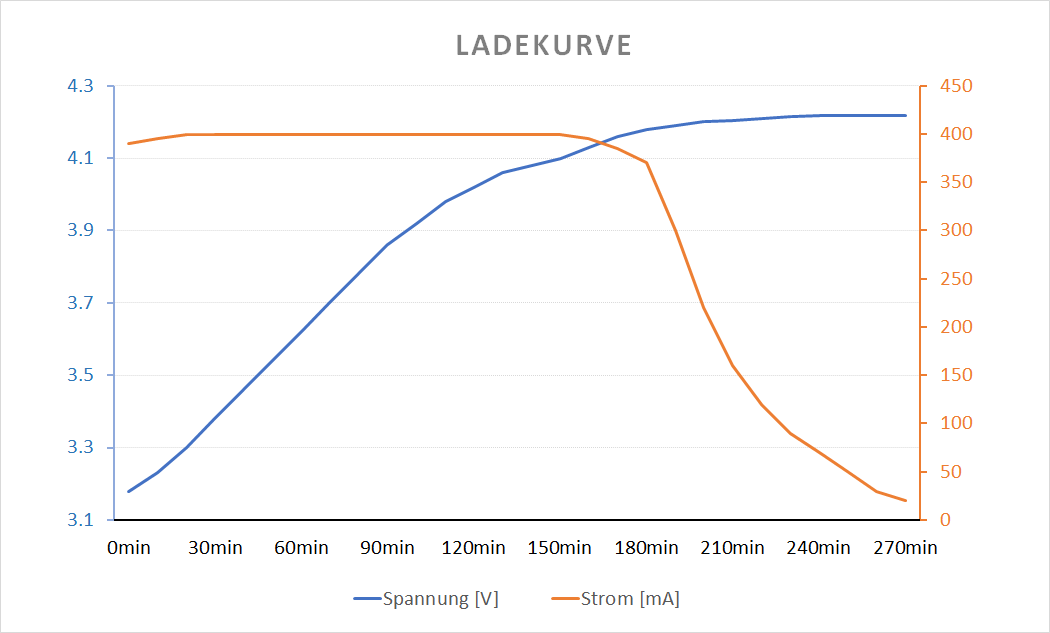
\includegraphics[width=120mm]{data/LadekurveEmmerich.png}
		\caption[Ladekurve Emmerich LI14500]{Ladekurve Emmerich LI14500} %picture caption
		\label{fig:LadekurveEmmerich}
	\end{center}
\end{figure}

Die oben genannten Vorgänge der Spannungs- und Stromregulierung sind in dieser Grafik gut ersichtlich, wobei der Ladevorgang nach dem erreichen von rund 20mA als fertig betrachtet wurde.

\subsubsection*{Induktive Ladeschaltung}\label{sec:batterie}
In diesem Abschnitt werden die Ergebnisse der induktiven Ladeschaltung präsentiert. Nachfolgend zeigt Abbildung \ref{fig:InduzierterStrom} die Abhängigkeit zwischen induziertem Strom und Spannung in Abhängigkeit zur Distanz z zwischen den Induktionsspulen.

\begin{figure}[H]
	\begin{center}
		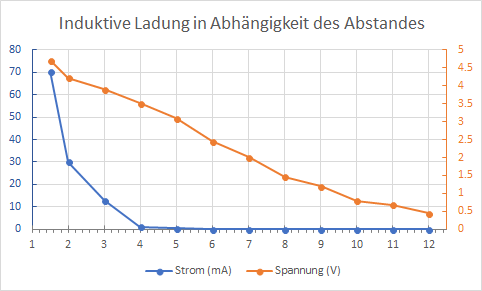
\includegraphics[width=100mm]{data/InduktiveLadung.png}
		\caption[Induzierter Strom in Abhängigkeit der Distanz]{Induzierter Strom in Abhängigkeit der Distanz} %picture caption
		\label{fig:InduzierterStrom}
	\end{center}
\end{figure}

In der Abbildung ist gut sichtbar, dass die Spannung fast linear zur Distanz abnimmt, hingegen der Ladestrom der Batterie extrem schnell klein wird. Aufgrund diesen Erkenntnissen sind wir gezwungen eine möglichst kurze Entfernung zwischen den Spulen einzuhalten. Deshalb wurde eine Ladestation entworfen, welche die bestmöglichen Induktionswerte garantiert. Der minimale Abstand welcher beim Ladezyklus erreicht werken kann beträgt rund $1.5mm$. Dieser Abstand entspricht ziemlich genau der Wanddicke des Dōjōs. Bei diesem Abstand resultiert ein Strom von maximal $70mA$, wobei die Ladezeit direkt von diesem Strom abhängt. Der Ladezyklus wird in zwei Etappen unterteilt. Bei der ersten Etappe wird die Batterie mit konstantem Strom geladen. Dies hat zur Folge, dass die Spannung von ihrem Minimalwert $3.3V$ auf den Schwellenwert von $4.2V$ reguliert wird. Um auf die notwendige Ladezeit des ersten Ladezyklus zu kommen, kann die Zeit während einer beliebig grossen Spannungsdifferenz gestoppt werden. Generell gilt: Umso grösser die Spannungsdifferenz, desto genauer die Approximation. Die Endzeit kann wie in nachfolgender Berechnung \ref{eq:LadezeitSpannungsregelung} linear hochgerechnet werden. Nachfolgend wird die Berechnung dieses Ladezyklus mit den Ladeströmen $I_{1}=30mA$ (schonender Zyklus), $I_{2}=50mA$ (normaler Zyklus) und $I_{3}=70mA$ (schneller Zyklus) veranschaulicht. 

\begin{equation}
\centering
t_{charge_{1.1}}=\frac{1.1 V}{(\frac{0.006 V}{10 Minuten})}=1'833.3 Minuten= 30h 33min
\label{eq:LadezeitSpannungsregelung1}
\end{equation}

\begin{equation}
\centering
t_{charge_{1.2}}=\frac{1.1 V}{(\frac{0.0016 V}{10 Minuten})}=687.5 Minuten= 11h 28min
\label{eq:LadezeitSpannungsregelung2}
\end{equation}

\begin{equation}
\centering
t_{charge_{1.3}}=\frac{1.1 V}{(\frac{0.0265 V}{10 Minuten})}=415.1 Minuten= 6h 55min
\label{eq:LadezeitSpannungsregelung3}
\end{equation}

Für die Spannungsregelung sind somit zwischen $30h$ und $7h$ Stunden notwendig. Da jedoch der Ladezyklus nach vollständiger Spannungsregelung noch nicht abgeschlossen ist, folgt noch die benötigte Zeit für die Stromregelung. Da diese nicht einfach berechnet werden kann, wurde dieser Prozess im Labor für alle drei Ströme durchgeführt und gestoppt. Es ergaben sich hierbei folgende Zeiten:
\begin{equation}
\centering
t_{charge_{2.1}}= 2h\space 7min
\label{eq:LadezeitStromregelung1}
\end{equation}

\begin{equation}
\centering
t_{charge_{2.2}}= 1h\space 18min
\label{eq:LadezeitStromregelung2}
\end{equation}

\begin{equation}
\centering
t_{charge_{2.3}}= 46min
\label{eq:LadezeitStromregelung3}
\end{equation}


Die gesamten Ladezeiten der beiden Ladezyklen ($t_{charge}=t_{charge_{1}}+t_{charge_{2}}$) betragen somit:\\

$t_{charge tot_{1}}=t_{charge_{1.1}}+t_{charge_{2.1}}=32h\space 27min \sim 32.5h$
 
$t_{charge tot_{2}}=t_{charge_{1.2}}+t_{charge_{2.2}}=12h\space 46min \sim 13h$
 
$t_{charge tot_{3}}=t_{charge_{1.3}}+t_{charge_{2.3}}=7h\space 41min \sim 8h$\\
\\
Die kurze Ladezeit von lediglich rund $8.7h$ ermöglicht ein schnelles aufladen. Da jedoch beim Ladezyklus mit einem Strom von $70mA$ sich die Spule mehr erwärmt als beim Ladezyklus mit $50mA$, wird vorgeschlagen, dass bei genügend Zeit der normale Zyklus mit $50mA$ gestartet wird. Dieser ist zwar um rund $4h$ langsamer, jedoch nachhaltiger für die eingebauten Materialien.

\subsubsection*{Inbetriebnahme der induktiven Ladeschaltung}\label{sec:erkenntnisse}

Der erste Prototyp der Pulsschaltung für die Induktion wurde mithilfe eines NE555 realisiert. Dabei wurden als Widerstände Potentiometer eingebaut, mit welchen die Resonanzfrequenz des LC-Gliedes gesucht werden sollte.

Der allererste Versuch ergab eine Übertragung von 5mA bei einer Taktfrequenz von 10kHz. Es stellte sich relativ schnell heraus, dass die Taktfrequenz viel zu tief war. Das konnte durch die Veränderung der Taktfrequenz der Pulsschaltung festgestellt werden. Bei höherer Taktfrequenz wurde die Übertragung besser.

Da die Taktfrequenz der NE555-Prototypenschaltung aufgrund der Wahl des Potentiometers auf $10kHz$ begrenzt war, wurde nun in weiteren Schritten mit dem Frequenzgenerator der $2n3055$ Leistungstransistor angesteuert. Des Weiteren wurde das C aus dem LC-Glied ausgebaut, um so das spezifische Maximum der Spule zu finden.

So wurde nun mit konstanter Eingangsspannung und variabler Taktfrequenz die Spule getestet. Mit höher werdender Frequenz wurde die Übertragung besser. Um diese noch weiter zu verbessern empfiehlt sich bei der Taktfrequenz einen Duty Cycle von möglichst $50\%$ zu erzielen.

Es erwies sich, dass bei der Taktfrequenz von $93kHz$ die beste Übertragung zustande kam. Bei höheren Frequenzen war diese wieder rückläufig. Da nun die optimale Frequenz gefunden und die Induktivität der Spule bekannt war ($14.9\mu H$), konnte der ideale Kopplungskondensator berechnet werden. Dies ergab, unter Berücksichtigung der E-Reihen, einen $220nF$ Kondensator als ideal. Damit die Spule nicht zu heiss werden und der Isolierlack nicht zu schmelzen beginnt, wurde der Strombegrenzungswiderstand des $2n2222$ mit $2\Omega$ definiert. Die Berechnung hierzu ist im oberen Text zu finden. Somit sind alle benötigten Bauteile bekannt.

\begin{figure}[H]
	\begin{center}
		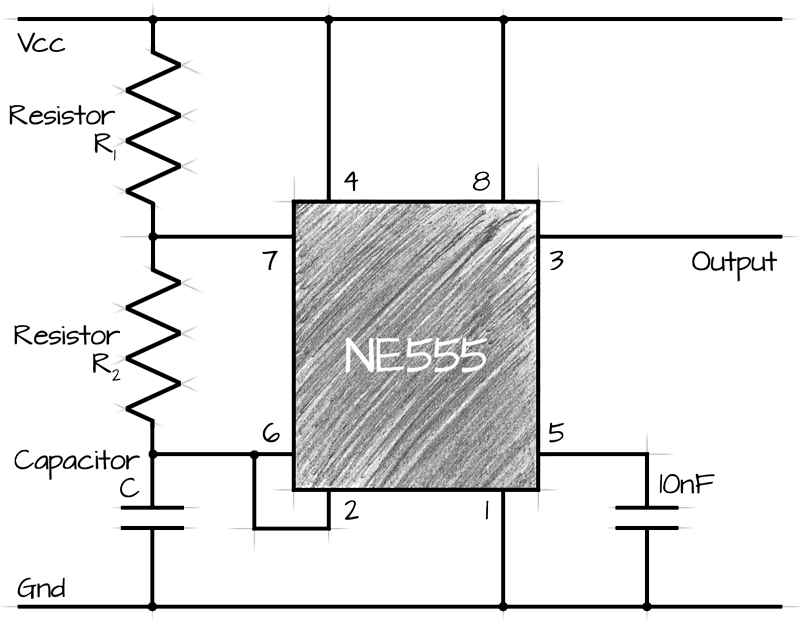
\includegraphics[width=80mm]{data/Ne555circuit.png}
		\caption[Verwendete Timerschaltung NE555 als Pulsquelle]{Verwendete Timerschaltung NE555 als Pulsquelle} %picture caption
		\label{fig:NE555}
	\end{center}
\end{figure}

$C = 1nF$\\
$R_{1} = 200\Omega$\\
$R_{2} = 9 k\Omega$\\

Mit diesen Werten konnte nach dem Gleichrichter, bei einer Übertragungsdistanz von einer Standard-Platinen dicke, eine Leerlaufspannung von ca. $17V$ und ein Kurzschlussstrom ca. 300mA gemessen werden. Es gilt jedoch zu beachten, dass diese Werte ohne Last gemessen wurden. 

Da nun die Induktionsstufe funktioniert wird diese nun um die Ladeschaltung erweitert. Hier ergab sich folgendes Problem:

Die Eingangsspannung des Lade-IC’s darf nicht mehr als $6.5$ Volt betragen. Da die Receiverspule sich im inneren des Dōjōs befindet und dadurch nur eine sehr geringe Baugrösse besitzen darf, kann diese zwangsläufig keine grossen Leistungen erbringen. Dies bedeutet, dass akzeptabel Ladeströme nur mit genügend hohen Spannungen erzeugt werden können.

Um dies zu erzielen wurde versucht, einen Spannungsregler einzubauen, um den übertragenen Strom bei zuhalten, jedoch die Spannung zu begrenzen. Das Ergebnis davon war jedoch ziemlich bescheiden. Der so entstehende Energieverlust ist ziemlich gross und ausserdem kam es vereinzelt vor, dass der Lade-IC trotzdem kaputt ging, da der Spannungsregler nicht sauber regelte. 

Die Ideale Lösung wäre natürlich einen geeigneteren Lade-IC zu nehmen. Da jedoch die Validierung desjenigen bereits durchgeführt wurde und nicht genügend Zeit vorhanden war diesen erneut zu bestellen wurde sich entschieden die Transceiver Schaltung ein wenig anzupassen.

Dabei gibt es folgende Möglichkeiten. Man kann die Eingangsspannung absenken. Dies beeinflusst jedoch auch den Übertragenen Strom exponentiell, da einerseits eingangsseitig mit weniger Spannung auch weniger Strom durch die Spule fliess und andererseits auch der Leistungsstransistor nicht sauber durchgesteuert wird da dieser ebenfalls an der gleichen Versorgungsspannung hängt und somit sein Pulssignal beeinflusst. Die zweite Möglichkeit ist die Taktfrequenz verringern. Dadurch wird die Induzierte Spannung ebenfalls abgesengt was ebenfalls den Strom exponentiell beeinflusst. Die dritte Möglichkeit wäre die Übertragungsdistanz zu verringern. Da aber sichergestellt werden wollte, dass der Dōjō-Boden dennoch eine gewisse Stabilität aufweisen sollte wurde diese Distanz der Platinendicke beigehalten.

Somit wurde die Schaltung lange ausgetestet um die beste Kombination zu erzielen. Das beste Resultat ergab die Kombination zwischen einer Taktfrequenz von ca 80kHz und einer Eingangs Spannung von $8.3V$. Dies lässt sich damit erklären das leichtes Absenken der beiden Möglichkeiten den Strom nicht so stark beeinflusst. Des Weiteren wurde der Strombegrenzungswiderstand auf $1.5\Omega$ verringert da sich die Eingangs Spannung verringert hat und ausserdem der Stromfluss durch die Spule damit erhöht wurde. 

Diese Anpassungen fielen ebenfalls zu Gunsten des Energiemanagements, jedoch ist dies eine stabile Variante für die ersten Prototypen. Durch die Anpassungen wird die überschüssige Energie in Form von Wärme an dem Transceiver Spule abgegeben. Die Test ergaben, dass so die Batterie bei einer Spannung von 4.7V mit 70mA geladen wird. Es ist ebenfalls möglich kurzzeitig mit einem höheren Strom zu laden, wenn die Eingangs Spannung nur geringfügig erhöht wird. (bis zu 120mA). Jedoch ist die Hitzeentwicklung hierbei so gross, dass nach einer gewissen Zeit die Übertragung zusammenbricht. Deshalb ist zu empfehlen die angegebenen Werte nicht zu überschreiten um eine dauernde Funktionalität zu gewährleisten.

Die Werte der oben beschriebenen angepassten Pulsschaltung sind folgende:\\
C: 1nF\\
R1: 200 $\Omega$\\
R2:9 k$\Omega$\\

\subsection{Testkonzept Software}\label{sec:testkonzeptSoftware}

Für einen einwandfreien Betrieb ist das Testing der Software einer der wichtigsten Bestandteile der Validierung. Dieses Kapitel wird in die Abschnitte \glqq PWM Signal\grqq, \glqq Verhalten der Statemachine\grqq, \glqq Kommunikation zwischen Bluetooth und Beacon\grqq wie auch \glqq Funktionalität der SD-Karte\grqq geteilt.

\subsubsection{PWM Signal}\label{sec: Validierung PWM Signal}

Das PWM Signal wurde mit dem Gleichen Signal wie das LC-Filter validiert. Dabei wurden sowohl die beiden PWM Kanäle mit dem KO aufgezeichnet wie in \ref{fig Signal PWM Ausgänge} zu sehen ist, sowie das gefilterte Signal. 

\begin{figure}[H]
	\begin{center}
		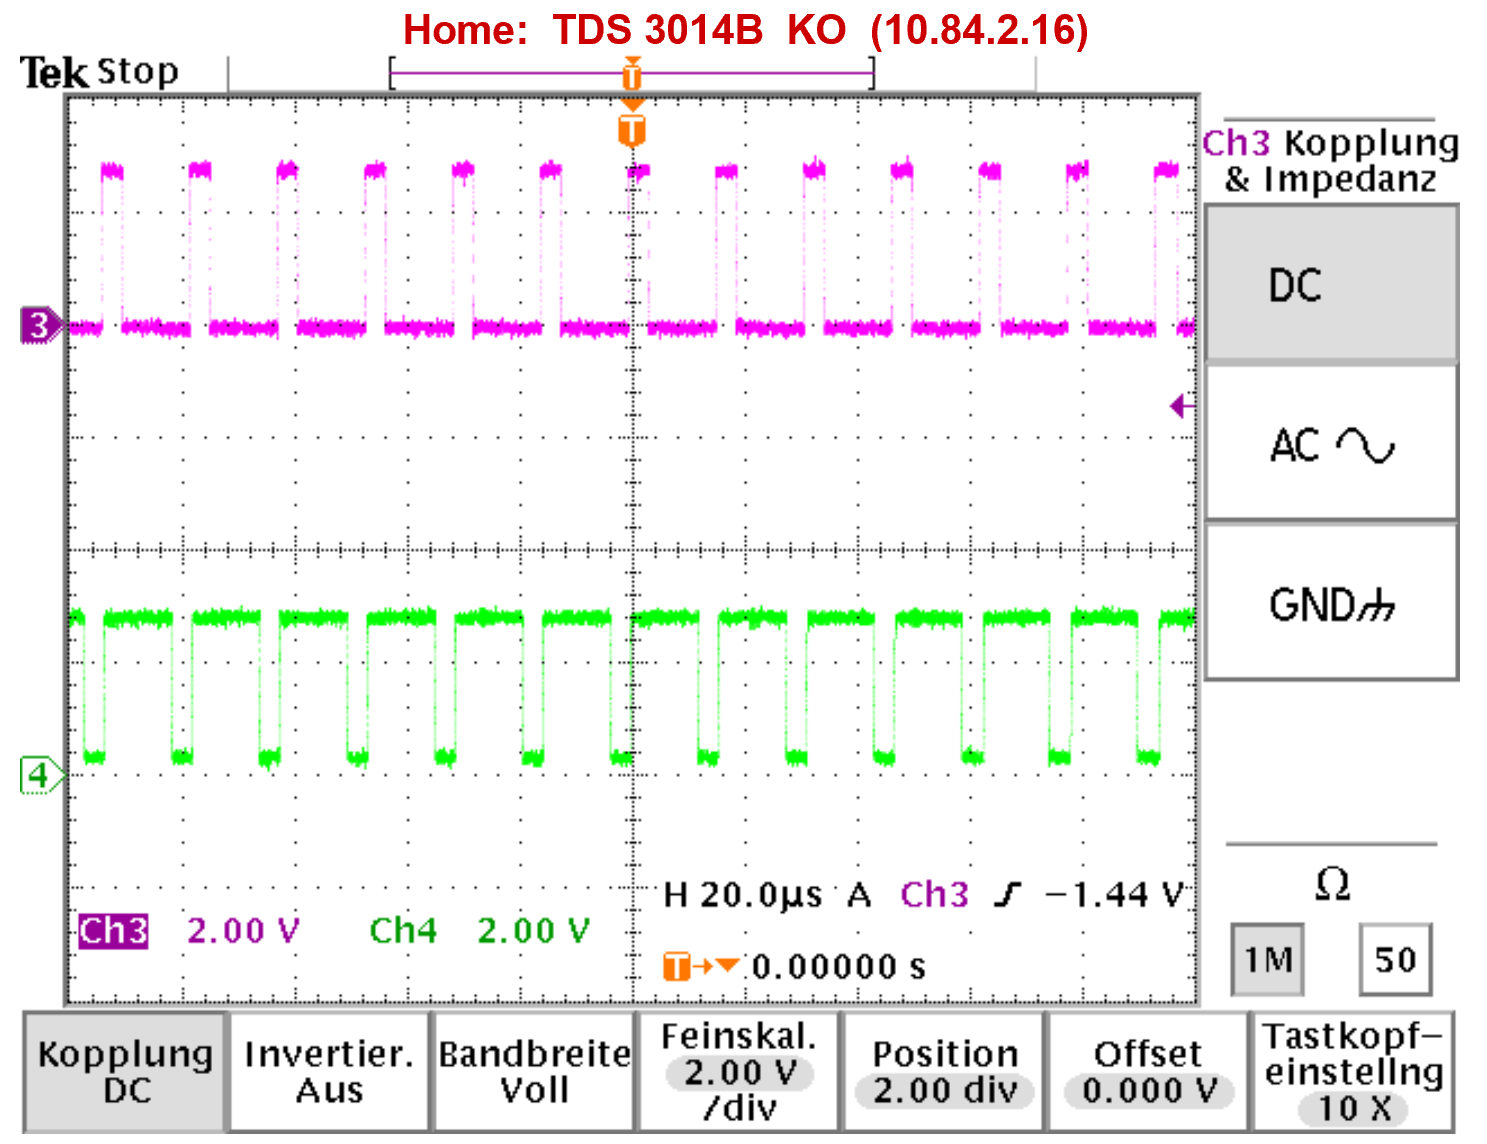
\includegraphics[width=120mm]{data/PWM_Signal_500Hz_Mono_mit_Infos.png}
		\caption[PWM Signal beider PWM Ausgänge]{PWM Signal beider PWM Ausgänge} %picture caption
		\label{fig:Signal PWM Ausgänge}
	\end{center}
\end{figure}


Aus \ref{fig:Signal PWM Ausgänge} ist ersichtlich, dass die beiden PWM Signale zwar invertiert zu einander stehen aber auch zeitlich (knapp knapp $4\mu s$) verschoben sind. Diese Zeitverschiebung hat jedoch keinen hörbaren Effekt und kann somit vernachlässigt werden.\\
Um die Einstellungen des PWM-Moduls aus \ref{sec:audioPWM} zu validieren, wurde ein $500Hz$ Sinus Signal mit dem KO abgebildet. Das entstandene Resultat ist in nachfolgender Abbildung \ref{fig:PWM Topval 500 Stereo} ersichtlich.

\begin{figure}[H]
	\begin{center}
		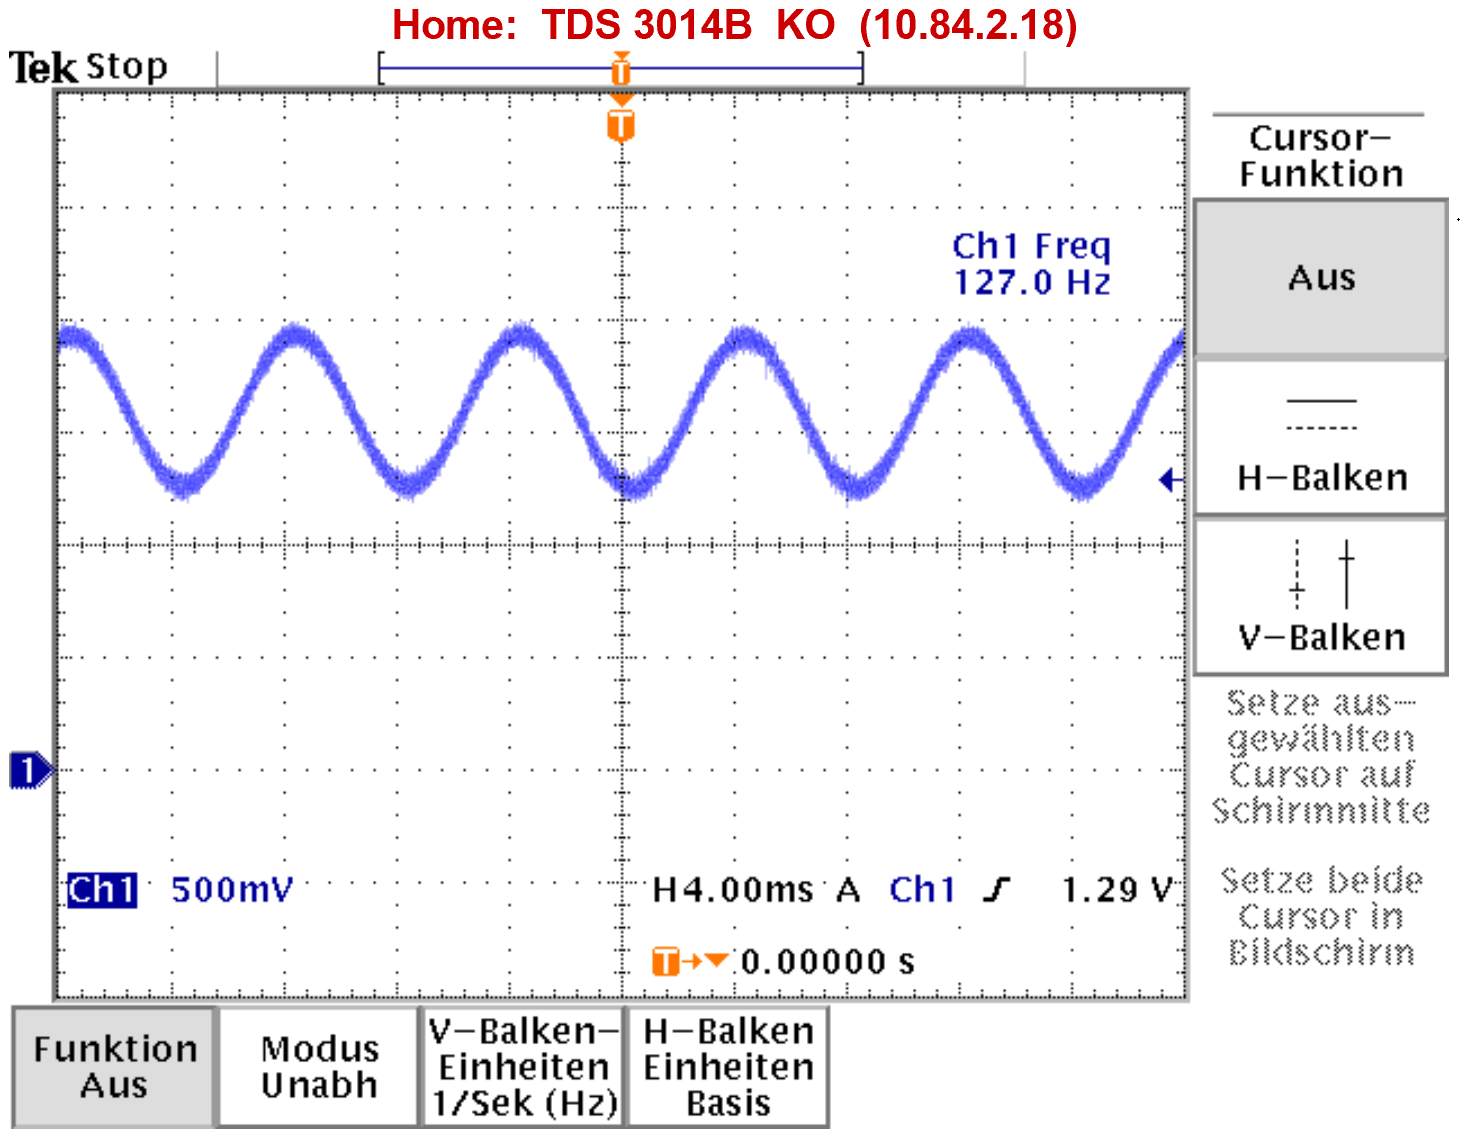
\includegraphics[width=120mm]{data/TOPVAL_Stereo_500.png}
		\caption[PWM auf $32kHz$ eingestellt]{PWM auf $32kHz$ eingestellt} %picture caption
		\label{fig:PWM Topval 500 Stereo}
	\end{center}
\end{figure}


Es ist augenfällig, dass die Frequenz des Signals nun nur $127Hz$ anstatt den angelegten $500Hz$ beträgt, war einem Faktor von rund $4$ entspricht. Um die gewünschten $500Hz$ zu erreichen, wurde der top value aus Kapitel \ref{sec:PWM initialisieren} von $500$ auf $125$ herunter gesetzt. Das entstandene Resultat ist in Abbildung \ref{fig:PWM Topval 125 Stereo} ersichtlich.

\begin{figure}[H]
	\begin{center}
		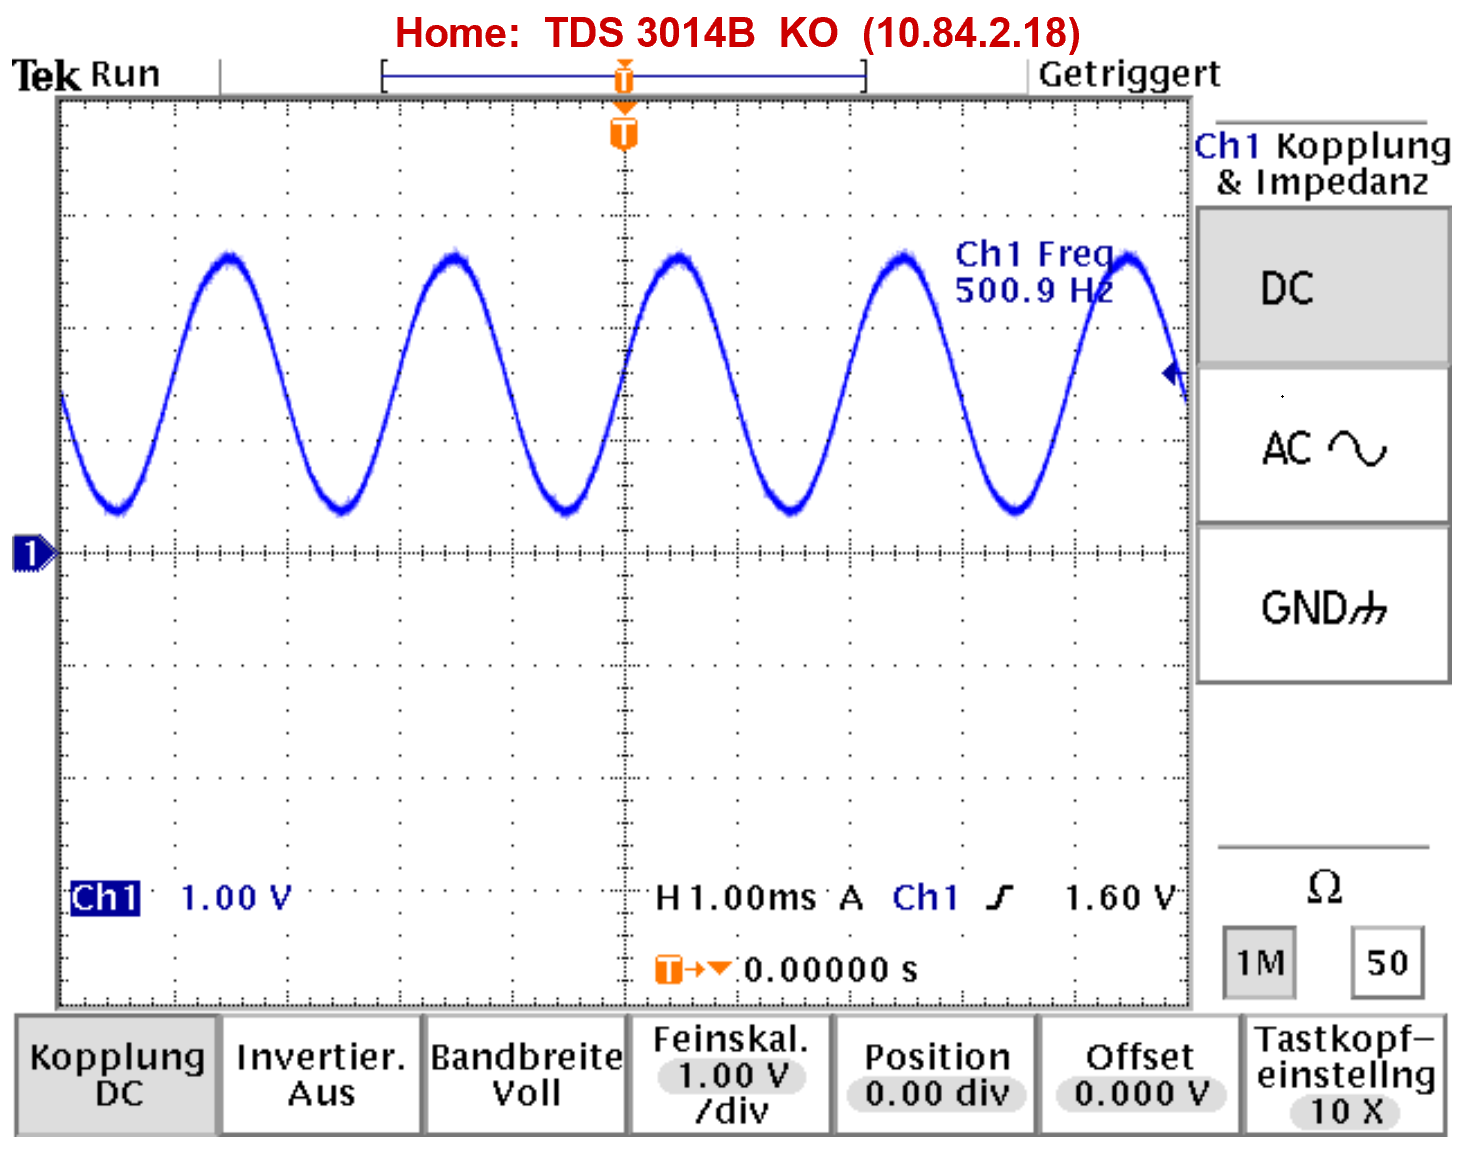
\includegraphics[width=120mm]{data/TOPVAL_Stereo_125.png}
		\caption[PWM auf $128kHz$ eingestellt]{PWM auf $128kHz$ eingestellt} %picture caption
		\label{fig:PWM Topval 125 Stereo}
	\end{center}
\end{figure}

Es ist ersichtlich, dass nun das Sinus Signal mit $500Hz$ schwingt. Da die Berechnungen einen top value von $500$ ergeben, deutet dies auf einen Fehler im Code, in der Audiodatei oder auf einen Überlegungsfehler hin. Es wurde herausgefunden, dass die Tests fälschlicherweise mit einer stereo Audiodatei durchgeführt wurden. Da jedoch nur ein Kanal angesteuert wird, ergibt sich ein Faktor $2$ unterschied zu den Berechnungen. Dieser Test wurde folglich noch einmal mit einer mono Audiodatei durchgeführt, wobei der top value gemäss unseren Erwartungen um den Faktor $2$ vom berechneten Wert abweicht.

\subsubsection{Statemachine}
Die Statemachine wurde auf ihr Verhalten hin getestet. Dabei wurden alle States mithilfe von Flags einmal erzwungen, wobei folgende States nicht korrekt funktionierten:

\begin{itemize}
	\item ADC-Batterie 
	\item Shutdown
	\item Merken Liste Löschen
	\item Charge
\end{itemize}

Es gilt anzumerken, dass diese \glqq fehlerhaften States\grqq in der Statemachiene eigentlich funktionieren, jedoch ihre Aufgabe nicht erfüllen können, da sie aus zeitlichen Gründen nicht implementiert wurden. Die Implementierung dieser States würden bei der Weiterverfolgung dieses Projektes als zusätzlicher Arbeitsschritt implementiert werden.

\subsubsection{Bluetooth}
Das Bluetooth Modul wurde mit verschiedenen Beacons getestet. Dabei is aufgefallen, dass bei der gleichzeitigen Verwendung von mehreren Beacons, welche mit unterschiedlichen Sendeintervallen senden, dies zu grösseren Problemen führt. Es dominieren die Beacons mit schnellerer Sendefrequenz, wobei die langsameren überblendet werden. Aus diesem Grund ist es zu empfehlen, dass die Abstände der Beacons gemäss Abbildung \ref{fig:ref_felder} angewendet werden. Die Radien können für jeden Beacon einzeln konfiguriert werden. Die grösse des Radius kann zwischen $0m$ und $40m$ varieren. Default mässig ist dieser Radius auf $3m$ eingestellt.

\begin{figure}[H]
	\begin{center}
		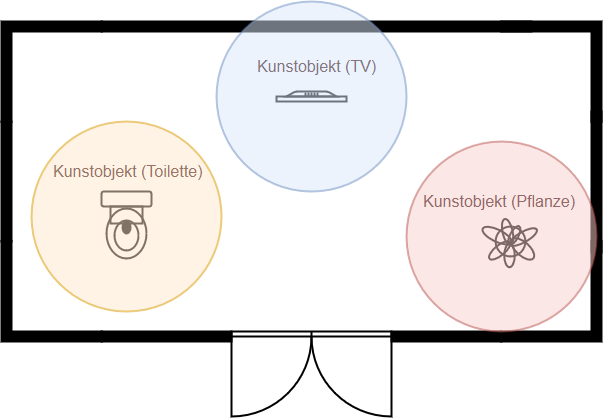
\includegraphics[width=120mm]{data/validierung_software_ref_felder.png}
		\caption[Überlappung der Referenz-Felder]{Überlappung der Referenz-Felder} %picture caption
		\label{fig:ref_felder}
	\end{center}
\end{figure}

\subsubsection{SD-Karte}
Das SD-Karten Modul hat alle Anforderungen erfüllt. Das lesen und schreiben ist problemlos möglich und funktionierte ohne weiteres. Einziger Makel weist die Funktion \glqq Merken\grqq (welche vom \glqq Like Button\grqq aufgerufen wird) auf. Hierbei ist es nicht möglich, ein gemerktes Kunstobjekt wieder zu löschen. Dafür ist es notwendig die SD-Karte aus dem Gerät zu nehmen und sie neu zu konfigurieren. Zudem kann man ein Kunstobjekt gleich mehrmals in die selbe \glqq Merkliste\grqq einfügen, was zwar keine Probleme im Gerät auslöst, aber vom Handlich her nicht sehr schön ist.



\newpage
\section{Schlusswort} \label{sec:schlusswort}

Dojo wurde ursprünglich in einem kleinen hohlen Stab konzeptioniert. In einer ersten Entwicklungsphase wurde ein Prototyp realisiert, welcher optisch an und für sich nichts mit dem Dojo zu tun hat. 

\newpage
\section{Ehrlichkeitserkl\"arung}
Ich bestätige mit der Unterschrift, dass der Bericht selbst verfasst und alle Quellen sauber und korrekt deklariert wurden.\\
\\
\\


\begin{tabular}{lp{23em}l}
 \hspace{3cm}   && \hspace{3cm} \\\cline{1-1}\cline{3-3}
 Ort, Datum     && Unterschrift Projektleiter
\end{tabular}

\newpage
\bibliographystyle{IEEEtran}
\bibliography{quelle}
\newpage
\listoffigures
\newpage
\begin{appendix}
\section{Anhang}\label{sec:anhang}

<<<<<<< HEAD
\subsection{Messresultate}\label{sec:messresultate}

\subsection{Lizenztexte}\label{sec:lizenztexte}

\begin{figure}[H]
	\begin{center}
		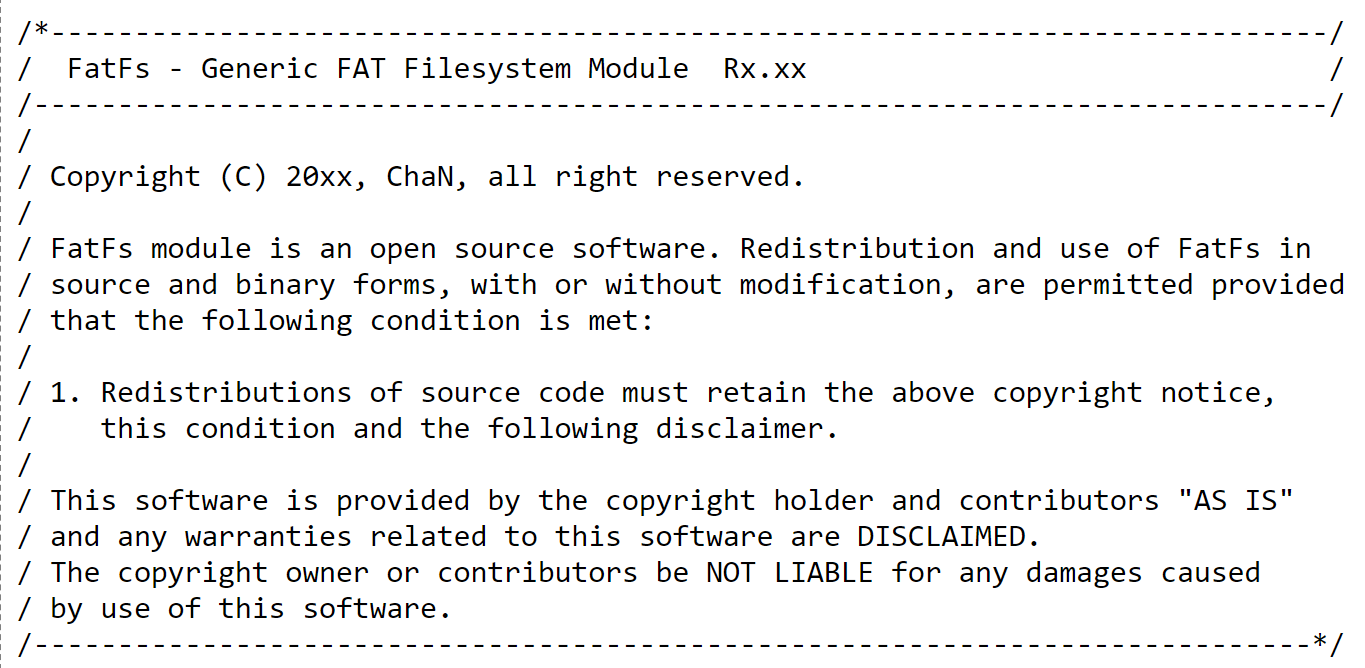
\includegraphics[width=0.7\textwidth]{data/Lizenztext_FatFs.png}
		\caption{Lizenztext FatFs library} %picture caption
		\label{fig:Lizentext FatFs}
	\end{center}
\end{figure}
=======
\newpage
\subsection{Lastenheft}\label{sec:lastenheft}

\includepdf{data/Lastenheft_EIT_P4_18FS_V2.pdf}
>>>>>>> a4eb713e28f4f560cfb29d75a0181608af44577d

\end{appendix}

%%%%%%%%%%%%%%%%%%%%%%%%%%%%%%%%%%%%%%%%%%%%%%%%%%%%%%%%
\end{document}

